\documentclass[degree=bachelor, fontset=custom, tocarialchapter]{thuthesis}
% 选项
%   degree=[bachelor|master|doctor|postdoctor], % 必选,学位类型
%   secret,                % 可选(默认:关闭),是否有密级
%   tocarialchapter,       % 可选(默认:关闭),章目录中使用黑体(这项表示同时打开下面两项)
%   tocarialchapterentry,  % 可选(默认:关闭),单独控制章标题在目录中使用黑体
%   tocarialchapterpage,   % 可选(默认:关闭),单独控制章页码在目录中使用黑体
%   pifootnote,            % 可选(默认:关闭),页脚编号采用 pifont 字体符号,建议打开

% 所有其它可能用到的包都统一放到这里了,可以根据自己的实际添加或者删除。
\usepackage{thuthesis}
\usepackage{float}
\newcolumntype{Y}{>{\centering\arraybackslash}X}

% 定义所有的图片文件在 figures 子目录下
\graphicspath{{figures/}}

% 可以在这里修改配置文件中的定义。导言区可以使用中文。
% \def\myname{薛瑞尼}

\begin{document}

%%% 封面部分
\frontmatter
\thusetup{
  %******************************
  % 注意:
  %   1. 配置里面不要出现空行
  %   2. 不需要的配置信息可以删除
  %******************************
  %
  %=====
  % 秘级
  %=====
  % secretlevel={秘密},
  % secretyear={10},
  %
  %=========
  % 中文信息
  %=========
  ctitle={基于开放通道SSD的高性能应用负载评测与优化},
  cdegree={工学学士},
  cdepartment={计算机科学与技术系},
  cmajor={计算机科学与技术},
  cauthor={孟垂正},
  csupervisor={舒继武教授},
  % cassosupervisor={陈文光教授}, % 副指导老师
  % ccosupervisor={某某某教授}, % 联合指导老师
  % 日期自动使用当前时间,若需指定按如下方式修改:
  % cdate={超新星纪元},
  %
  % 博士后专有部分
  % cfirstdiscipline={计算机科学与技术},
  % cseconddiscipline={系统结构},
  % postdoctordate={2009年7月——2011年7月},
  % id={编号}, % 可以留空: id={},
  % udc={UDC}, % 可以留空
  % catalognumber={分类号}, % 可以留空
  %
  %=========
  % 英文信息
  %=========
  % etitle={Ji yu kai fang tong dao SSD},
  % 这块比较复杂,需要分情况讨论:
  % 1. 学术型硕士
  %    edegree:必须为Master of Arts或Master of Science(注意大小写)
  %             “哲学、文学、历史学、法学、教育学、艺术学门类,公共管理学科
  %              填写Master of Arts,其它填写Master of Science”
  %    emajor:“获得一级学科授权的学科填写一级学科名称,其它填写二级学科名称”
  % 2. 专业型硕士
  %    edegree:“填写专业学位英文名称全称”
  %    emajor:“工程硕士填写工程领域,其它专业学位不填写此项”
  % 3. 学术型博士
  %    edegree:Doctor of Philosophy(注意大小写)
  %    emajor:“获得一级学科授权的学科填写一级学科名称,其它填写二级学科名称”
  % 4. 专业型博士
  %    edegree:“填写专业学位英文名称全称”
  %    emajor:不填写此项
  edegree={Bachelor of Engineering},
  emajor={Computer Science and Technology},
  eauthor={Chuizheng Meng},
  esupervisor={Professor Shu Jiwu},
  % eassosupervisor={Chen Wenguang},
  % 日期自动生成,若需指定按如下方式修改:
  % edate={December, 2005}
  %
  % 关键词用“英文逗号”分割
  ckeywords={开放通道SSD,高性能应用,超级块映射},
  ekeywords={open-channel ssd,high performance computing application,super-block mapping}
}

% 定义中英文摘要和关键字
\begin{cabstract}
  本文主要研究在开放通道SSD上利用高性能应用的IO负载特性优化其IO性能的问题。高性能应用的IO负载具有IO请求地址按页对齐,负载中覆盖写比例很高的特点。具有这种特点的IO序列在SSD上会产生大量不含有任何脏页的无效数据块,回收时可直接擦除而无需重新写入脏页。现有方法采用的页粒度的地址映射高度灵活性的优势在这种负载下无法发挥,反而徒然增加了映射表维护的开销。本文提出的基于超级块粒度地址映射的优化方法减少了这一不必要的开销,同时维持了与现有方法相近的吞吐性能。实验表明,本文采用的超级块映射-贪心垃圾回收方法能够利用更小的映射表和更低的映射表维护成本达到与现有方法相近的IO性能。

  本文的工作主要有:
  \begin{itemize}
    \item 抓取了典型高性能计算应用LAMMPS和MACDRP的IO负载记录并分析了二者的负载特征;
    \item 在用户态实现了多种IO优化策略与相应的评测程序;
    \item 将现有方法页粒度的地址映射改进为超级块粒度的映射,在保证IO性能不下降的同时大幅减少了映射表体积和维护开销。
  \end{itemize}
\end{cabstract}

% 如果习惯关键字跟在摘要文字后面,可以用直接命令来设置,如下:
% \ckeywords{\TeX, \LaTeX, CJK, 模板, 论文}

\begin{eabstract}
  This article focuses on optimizing the IO performance of an open channel SSD using high-performance application IO load characteristics. In the IO load of high-performance applications, the IO request address is page-aligned and the load has a high write-to-write ratio. An IO sequence with these characteristics will produce a large number of invalid data blocks on the SSD that do not contain any dirty pages, which can be erased directly with no dirty page requiring rewritting. The page-granularity address mapping used by the existing method cannot enjoy the benefit of its flexibility under such a load, but in turn increases the overhead of maintaining the mapping table. The optimization method based on super-block granularity address mapping proposed in this paper reduces this unnecessary overhead while maintaining similar throughput performance to the existing method. Experiments show that the proposed method can use a smaller map and a lower map maintenance cost to achieve similar IO performance to the existing method.

  The work of the paper includes:
  \begin{itemize}
    \item Tracking the IO load of two high-performance computing applications and analyzing characteristics of their IO records;
    \item Implementing multiple optimization strategies and corresponding benchmark tools;
    \item Modifying page-granularity address mapping in the existing method to super-block granularity address mapping, which reduces the size and the maintaining cost of the mapping table while keeping the IO performance.
  \end{itemize}
\end{eabstract}

% \ekeywords{\TeX, \LaTeX, CJK, template, thesis}

% 如果使用授权说明扫描页,将可选参数中指定为扫描得到的 PDF 文件名,例如:
% \makecover[scan-auth.pdf]
\makecover

%% 目录
\tableofcontents

%% 符号对照表
% \begin{denotation}[3cm]
\item[HPC] 高性能计算 (High Performance Computing)
\item[cluster] 集群
\item[Itanium] 安腾
\item[SMP] 对称多处理
\item[API] 应用程序编程接口
\item[PI] 聚酰亚胺
\item[MPI] 聚酰亚胺模型化合物,N-苯基邻苯酰亚胺
\item[PBI] 聚苯并咪唑
\item[MPBI] 聚苯并咪唑模型化合物,N-苯基苯并咪唑
\item[PY] 聚吡咙
\item[PMDA-BDA]	均苯四酸二酐与联苯四胺合成的聚吡咙薄膜
\item[$\Delta G$] 活化自由能 (Activation Free Energy)
\item[$\chi$] 传输系数 (Transmission Coefficient)
\item[$E$] 能量
\item[$m$] 质量
\item[$c$] 光速
\item[$P$] 概率
\item[$T$] 时间
\item[$v$] 速度
\item[劝学] 君子曰:学不可以已。青,取之于蓝,而青于蓝;冰,水为之,而寒于水。木
  直中绳。輮以为轮,其曲中规。虽有槁暴,不复挺者,輮使之然也。故木受绳则直,金就
  砺则利,君子博学而日参省乎己,则知明而行无过矣。吾尝终日而思矣,不如须臾之所学
  也;吾尝跂而望矣,不如登高之博见也。登高而招,臂非加长也,而见者远;顺风而呼,
  声非加疾也,而闻者彰。假舆马者,非利足也,而致千里;假舟楫者,非能水也,而绝江
  河,君子生非异也,善假于物也。积土成山,风雨兴焉;积水成渊,蛟龙生焉;积善成德,
  而神明自得,圣心备焉。故不积跬步,无以至千里;不积小流,无以成江海。骐骥一跃,
  不能十步;驽马十驾,功在不舍。锲而舍之,朽木不折;锲而不舍,金石可镂。蚓无爪牙
  之利,筋骨之强,上食埃土,下饮黄泉,用心一也。蟹六跪而二螯,非蛇鳝之穴无可寄托
  者,用心躁也。—— 荀况
\end{denotation}



%%% 正文部分
\mainmatter
\chapter{引言}
\label{cha:intro}

\section{研究动机}

\section{相关工作}

\section{主要工作}

\chapter{开放通道SSD与高性能应用}
\label{cha:ssd_hpc}

\section{开放通道SSD设备简介}
\subsection{SSD内部结构}
SSD,全称为固态硬盘(solid-state drive),是一种由多个闪存芯片组成的存储设备。本文主要关注由NAND闪存芯片组成的SSD,因为目前主流的SSD设备均采用NAND芯片,对NAND的管理与现实应用关系更加密切。

典型SSD设备的内部结构如图\ref{fig:ssd_geo}所示。SSD的控制器上并行连接了多组闪存芯片,每组闪存芯片一般包含数十个NAND存储芯片,并通过名为Channel的结构连接到控制器。每个Channel下的芯片按照Die、Plane、Block和Page的层级组织。一个Die每次只允许执行一个IO请求,即SSD并行执行IO请求的最小单元是Die。在开放通道SSD设备中,一个或者多个Die也会被合并称为一个Lun。每个Die含有相同数量的Plane,同样,每个Plane含有相同数量的Block,每个Block也含有相同数量的Page。每个Page还继续被分为固定大小的Sector,同时包含一个OOB区域(out-of-bound area)用于存储元数据。

\begin{figure}[H]
  \centering
  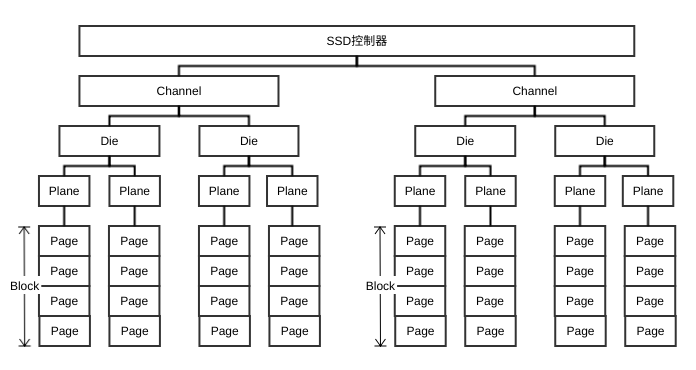
\includegraphics[width=0.8\textwidth]{ssdgeo.png}
  \caption{SSD设备的内部结构}
  \label{fig:ssd_geo}
\end{figure}

\subsection{SSD读写操作的限制}
和传统磁盘相比,尽管SSD有随机访问迅速的优势,其读写操作有一些额外的限制:

\begin{enumerate}[1.]
\item 任何一个页(Page)在写入或者再次写入前必须经过擦除操作。
\item SSD读写操作的最小单位为页(Page),而擦除操作的最小单位是块(Block)。
\item 闪存芯片可被擦除的次数是有限的。对于TLC/QLC类型的芯片,其可经受的擦除循环数数量级在$10^2$,而对于MLC和QLC芯片,这一数值的数量级分别为$10^3$和$10^5$。
\end{enumerate}

这些限制使得SSD设备在覆盖写入已有数据的区域时不能像传统磁盘一样就地写入。这种做法会导致被覆盖写位置所在的整个块被擦除,而为了保证未被覆盖的有效数据得到保留,位于同一块内但没有被覆盖写的数据需要先被读入缓存后在擦除完成后重新写入。这就增加了额外写操作,使得写入效率大幅下降。可行的做法是如非必要则不去真正清除被覆盖写的数据,而是将其标记为无效,同时在设备上为新写入的数据分配一块新空间。这种做法会导致同一个逻辑地址在多次写入时对应的物理地址发生变化,因此需要建立逻辑地址到物理地址的映射方式。同时,被标记为无效的数据所占用空间需要定期进行释放,否则整个设备的可写入量将远远小于实际容量,因此需要设计垃圾回收算法以回收空间。由于芯片存在最大擦除次数的限制,映射方式和垃圾回收算法需要确保设备所有块的被擦除次数尽量均匀,否则被擦除次数较多的块将在达到其最大擦除次数限制后损坏,导致设备可用空间下降。SSD设备内部设计了闪存转换层(FTL,Flash Translation Layer)实现以上地址映射、垃圾回收和负载均衡的功能。

\subsection{开放通道SSD简介}
开放通道SSD(Open-Channel SSD)是近年新出现的一种SSD设备。与传统SSD设备相比,开放通道SSD的特点是外部程序可直接控制其内部结构的读写,从而允许主机控制数据的分布和进行物理IO调度;而传统SSD设备仅对外暴露块设备的接口,外部程序很难获知其内部的闪存转换层是如何将系统对块设备的操作转换为对内部结构的操作的。

\section{高性能应用的IO特征分析}
这里选择LAMMPS和MACDRP两种高性能应用,采集它们运行一段时间内的IO Trace并分析其特点。由于2种应用运行时会向不同的主机写入数据,且经汇总发现对于IO操作数最多的前10台主机其IO特征高度一致,故以下分析时只取其中操作数最多的一台主机上的IO Trace进行分析。
\subsection{LAMMPS应用的IO特征分析}
LAMMPS的全称为大规模原子/分子大量并行模拟器。它能够并行模拟原子、中观或者连续体尺度上的大规模粒子行为。

\begin{figure}[H]
  \centering
  \subcaptionbox{LAMMPS的IO Trace\label{fig:iotrace_lammps}}
    {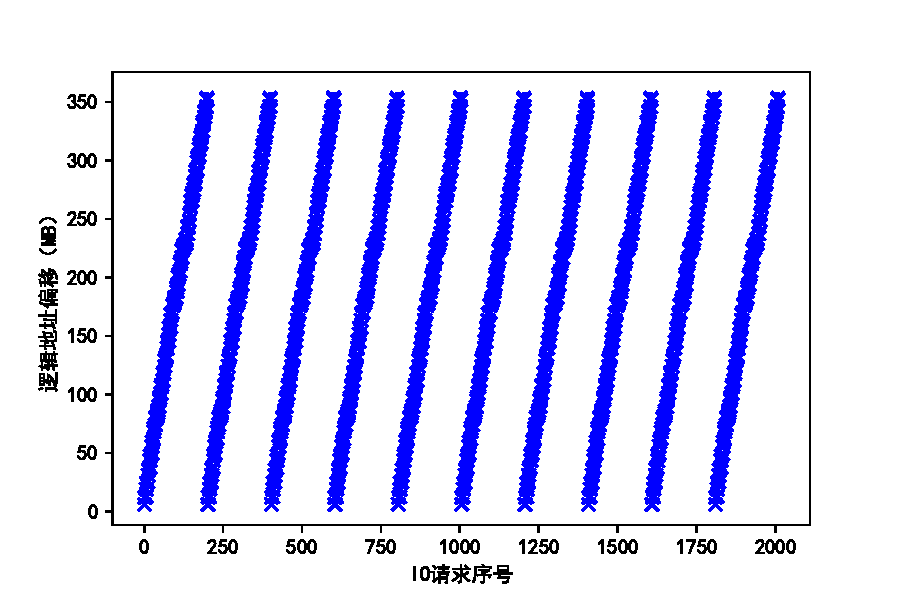
\includegraphics[width=0.4\textwidth]{iotrace_lammps.pdf}}
  \hspace{4em}
  \subcaptionbox{LAMMPS的IO Trace(部分)\label{fig:iotrace_lammps_sub}}
      {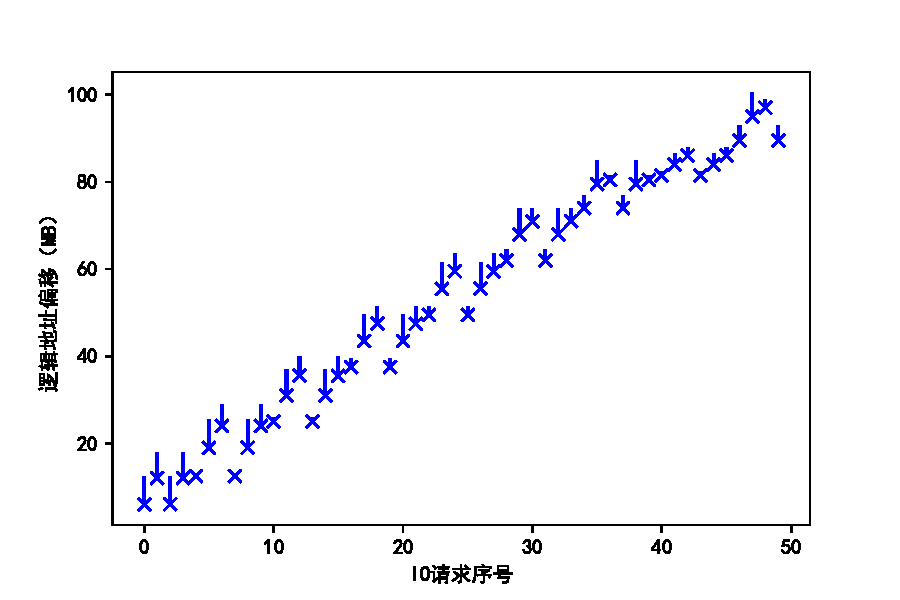
\includegraphics[width=0.4\textwidth]{iotrace_lammps_sub.pdf}}
  \caption{LAMMPS的IO Trace}
  \label{fig:iotrace_lammps_all}
\end{figure}

图\ref{fig:iotrace_lammps_all}展示了LAMMPS的IO Trace,采集到的IO Trace全部请求均为写请求。如图\ref{fig:iotrace_lammps},LAMMPS对逻辑地址范围0-358MB内的空间反复写入。图\ref{fig:iotrace_lammps_sub}为对其中一段IO Trace放大显示的结果,其中x表示IO请求的起始位置,铅直线覆盖部分表示IO请求涉及的逻辑地址空间。可以观察到LAMMPS对同一段空间进行了多次写操作。统计得到LAMMPS的这段IO Trace共写入了7075MB的数据,而访问的逻辑地址最大仅为358MB,显然这一过程中存在大量的覆盖写操作。

\begin{figure}[H]
  \centering
  \subcaptionbox{LAMMPS的IO请求数据量累积分布函数\label{fig:iotrace_lammps_iosize_cdf}}
    {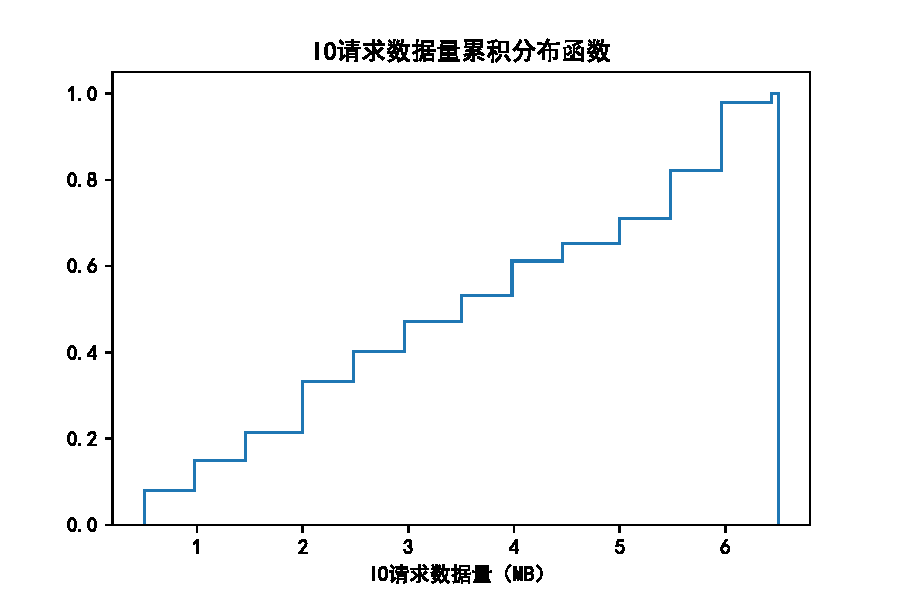
\includegraphics[width=0.25\textwidth]{iotrace_lammps_iosize_cdf.pdf}}
  \hspace{1em}
  \subcaptionbox{LAMMPS的IO请求起始地址页内偏移量累积分布函数\label{fig:iotrace_lammps_iostart_cdf}}
      {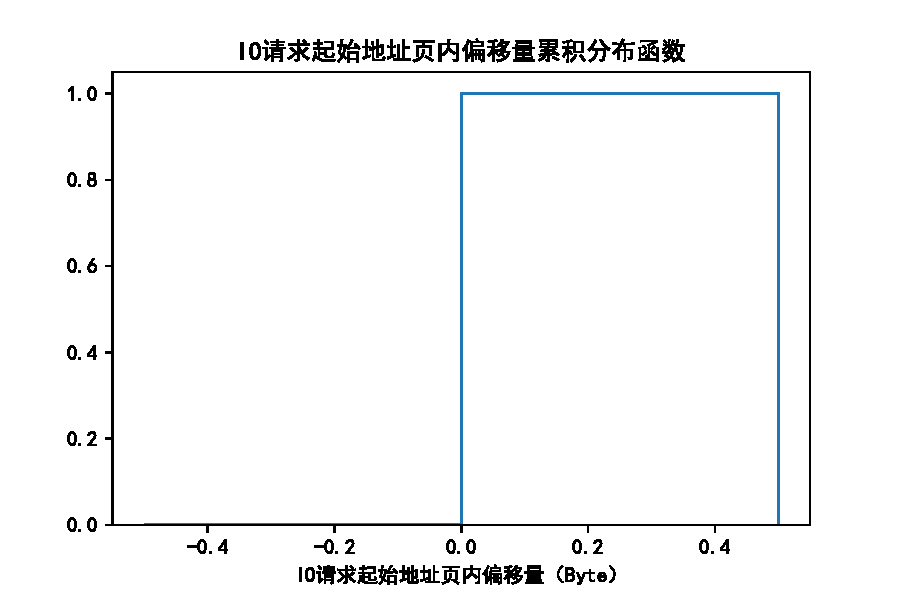
\includegraphics[width=0.25\textwidth]{iotrace_lammps_iostart_cdf.pdf}}
      \hspace{1em}
      \subcaptionbox{LAMMPS的IO请求结束地址页内偏移量累积分布函数\label{fig:iotrace_lammps_ioend_cdf}}
          {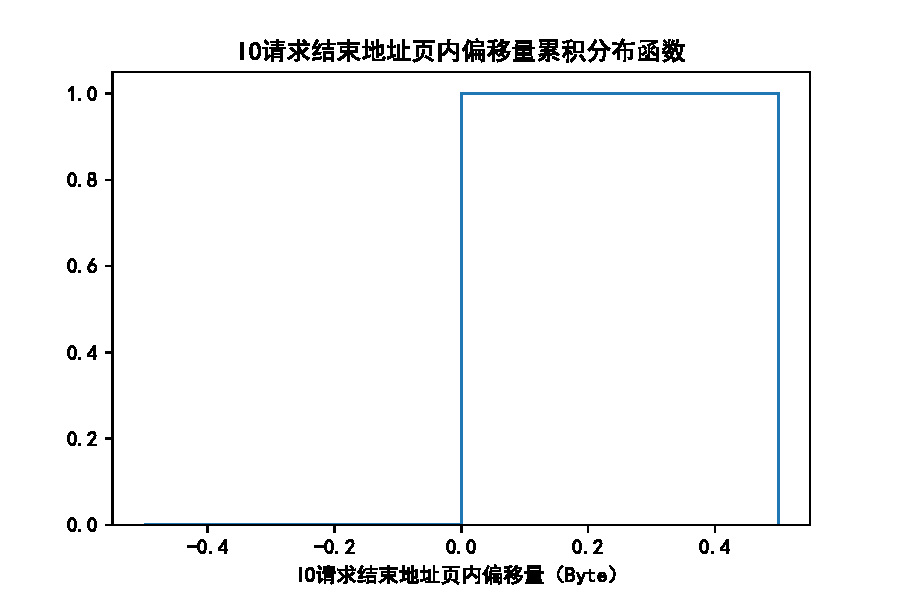
\includegraphics[width=0.25\textwidth]{iotrace_lammps_ioend_cdf.pdf}}
  \caption{LAMMPS的IO请求按页对齐情况}
  \label{fig:iotrace_lammps_iocdf}
\end{figure}
图\ref{fig:iotrace_lammps_iocdf}展示了LAMMPS的IO请求按页对齐的情况。这里的页大小取为后续实验使用的SSD页大小32768KB。如图\ref{fig:iotrace_lammps_iosize_cdf},几乎所有的IO请求大小都大于500KB。如图\ref{fig:iotrace_lammps_iostart_cdf}和图\ref{fig:iotrace_lammps_ioend_cdf},全部的IO请求起始地址和结束地址都对齐到页,同时表明IO请求的大小也按页对齐。

\subsection{MACDRP应用的IO特征分析}
\label{ssc:ioana}
MACDRP能够模拟地震波在具有足够精度地表地形下的传播效果。
\begin{figure}[H]
  \centering
  \subcaptionbox{MACDRP的IO Trace\label{fig:iotrace_macdrp}}
    {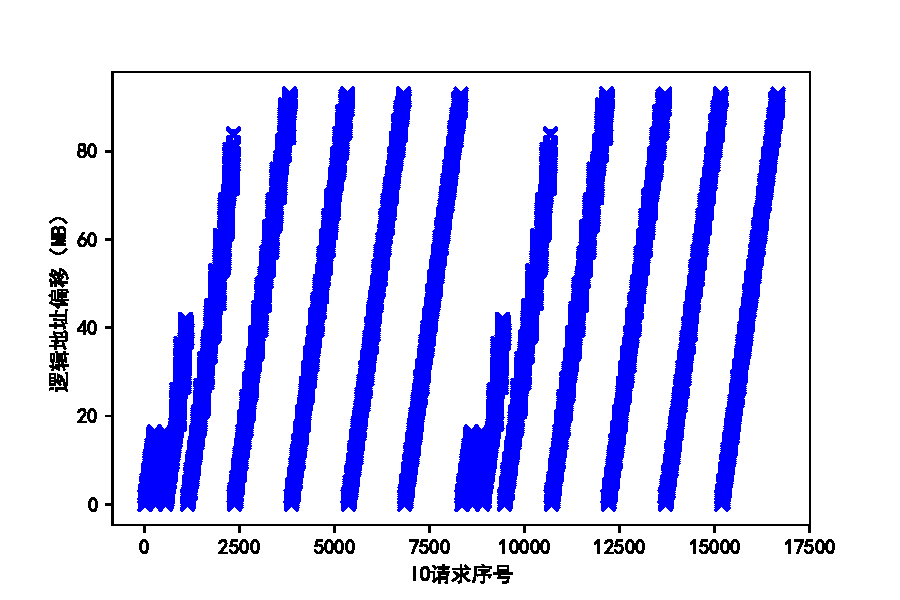
\includegraphics[width=0.4\textwidth]{iotrace_macdrp.pdf}}
  \hspace{4em}
  \subcaptionbox{MACDRP的IO Trace(部分)\label{fig:iotrace_macdrp_sub}}
      {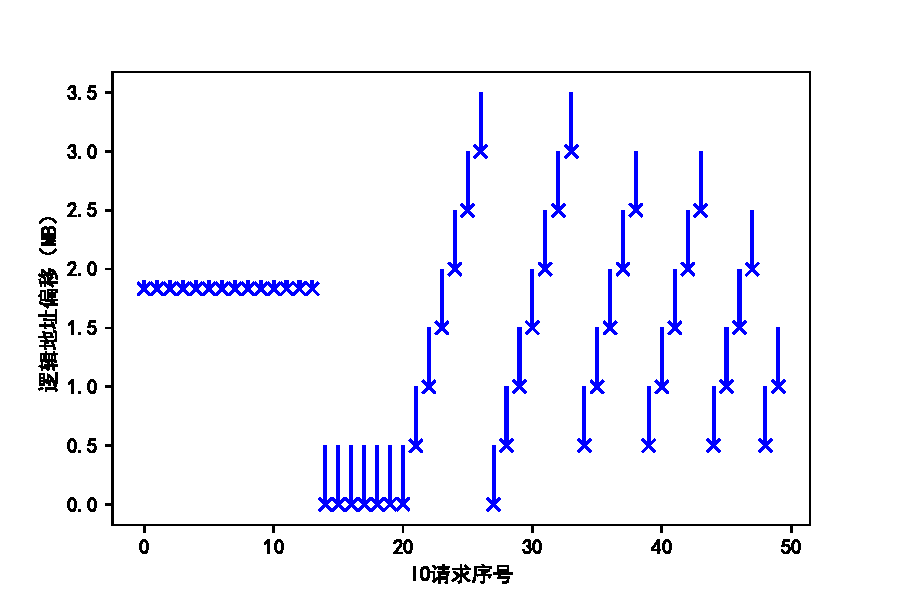
\includegraphics[width=0.4\textwidth]{iotrace_macdrp_sub.pdf}}
  \caption{MACDRP的IO Trace}
  \label{fig:iotrace_macdrp_all}
\end{figure}
图\ref{fig:iotrace_macdrp_all}展示了MACDRP的IO Trace,采集到的IO Trace全部请求均为写请求。与LAMMPS的情况类似,MACDRP同样在有限的逻辑地址空间内进行了大量覆盖写操作。如图\ref{fig:iotrace_macdrp},MACDRP在逻辑地址范围0-93MB内的空间反复写入了高达8256MB的数据。图\ref{fig:iotrace_macdrp_sub}为对其中一段IO Trace放大显示的结果,符号含义与图\ref{fig:iotrace_lammps_sub}相同。可以观察到MACDRP对同一段空间进行了高达7次写操作。这一过程中覆盖写的比例比LAMMPS更高。

\begin{figure}[H]
  \centering
  \subcaptionbox{MACDRP的IO请求数据量累积分布函数\label{fig:iotrace_macdrp_iosize_cdf}}
    {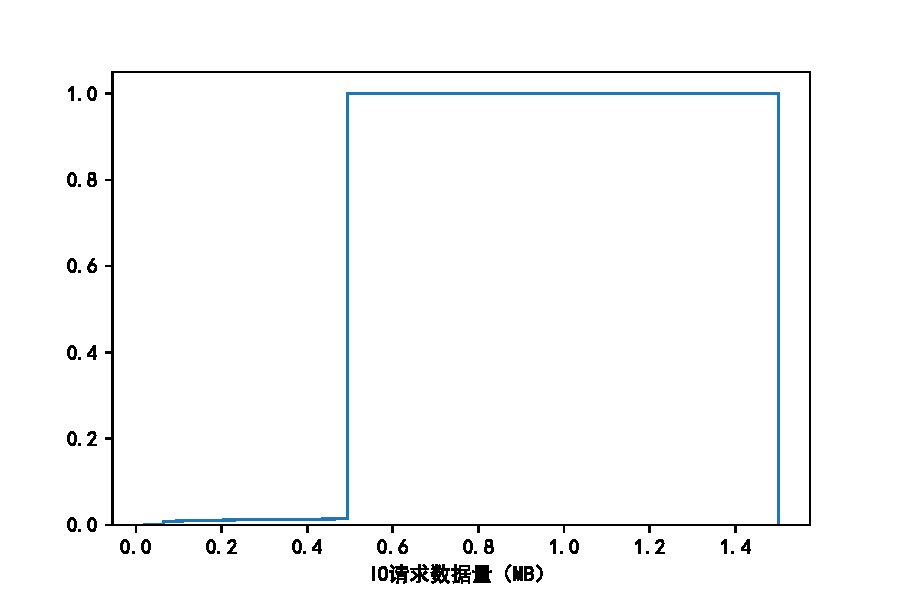
\includegraphics[width=0.25\textwidth]{iotrace_macdrp_iosize_cdf.pdf}}
  \hspace{1em}
  \subcaptionbox{MACDRP的IO请求起始地址页内偏移量累积分布函数\label{fig:iotrace_macdrp_iostart_cdf}}
      {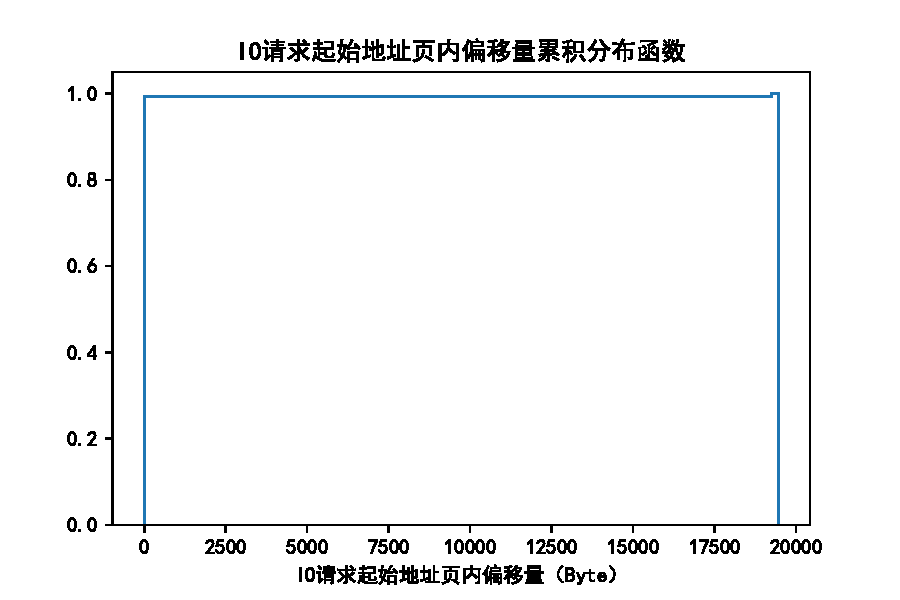
\includegraphics[width=0.25\textwidth]{iotrace_macdrp_iostart_cdf.pdf}}
      \hspace{1em}
      \subcaptionbox{MACDRP的IO请求结束地址页内偏移量累积分布函数\label{fig:iotrace_macdrp_ioend_cdf}}
          {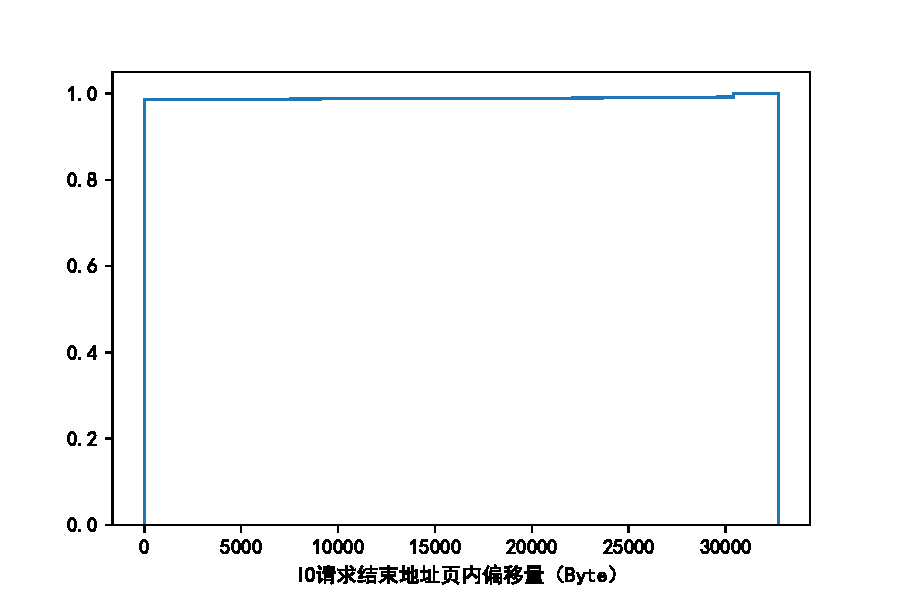
\includegraphics[width=0.25\textwidth]{iotrace_macdrp_ioend_cdf.pdf}}
  \caption{MACDRP的IO请求按页对齐情况}
  \label{fig:iotrace_macdrp_iocdf}
\end{figure}

图\ref{fig:iotrace_macdrp_iocdf}显示了MACDRP的IO请求按页对齐的情况。由图\ref{fig:iotrace_macdrp_iostart_cdf}和图\ref{fig:iotrace_macdrp_ioend_cdf}可知,其绝大部分IO请求都能按页对齐,仅有少量请求的开始/结束地址页内偏移量不为0。图\ref{fig:iotrace_macdrp_iosize_cdf}表明MACDRP的几乎所有IO请求数据量大小均相同,为512KB。

根据以上的分析,可以发现所选高性能应用的IO负载具有覆盖写比例高、请求按页对齐、一次请求写入的数据量恰好为整数页的特点。这样的负载在写入时必然会在过程中创造大量连续的无效数据区域,这些区域在被垃圾回收时可以直接擦除而无需重新写入脏页。根据这一特点,可以尝试简化现有闪存转换层的垃圾回收算法,或者简化其映射方式。

\section{本章小结}
本章首先介绍实验所用的开放通道SSD设备的内部结构、读写特点以及其定制性强的优势,然后分析了LAMMPS和MACDRP两种高性能应用IO负载的特征,并探讨了根据其特征对闪存转换层进行优化的可能性。
\chapter{优化设计与实现}
\label{cha:imple}

\section{开放通道SSD访问}
\subsection{访问流程}
传统SSD的访问方式如图\ref{fig:imple_traditional_ssd}所示。用户态程序发出的文件操作请求经内核的虚拟文件系统和物理文件系统处理后,物理文件系统将请求转换为对块设备的读写操作。传统SSD设备内部设置的闪存转换层(Flash Translation Layer)对外提供了与块设备兼容的接口,使得原本为块设备设计的文件系统能够在SSD上直接使用;闪存转换层对内负责处理逻辑地址到物理地址的映射、垃圾回收和负载均衡工作,将对块设备的请求转换为对闪存芯片的读、写和擦除操作。

开放通道SSD的访问方式如图\ref{fig:imple_ocssd},用户态程序可以通过liblightnvm库\footnote{https://github.com/OpenChannelSSD/liblightnvm}对SSD内部结构进行直接访问,从而无需经过文件系统和闪存转换层。在这种访问方式下,用户态程序可以模拟出闪存转换层需要提供的映射、垃圾回收和负载均衡功能,并能够根据自身IO特征进行适当的优化。

\begin{figure}[H]
    \centering
    \subcaptionbox{传统SSD的访问流程\label{fig:imple_traditional_ssd}}
      {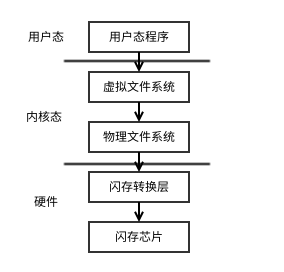
\includegraphics[width=0.4\textwidth]{traditional_ssd.png}}
    \hspace{4em}
    \subcaptionbox{开放通道SSD的访问流程\label{fig:imple_ocssd}}
        {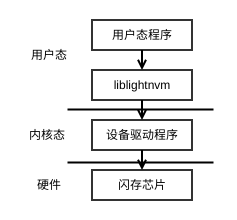
\includegraphics[width=0.4\textwidth]{ocssd.png}}
    \caption{两种SSD的访问流程}
    \label{fig:imple_ssdvisit}
\end{figure}

具体到本文的实现,由于可供评测的数据为高性能应用运行时文件系统下发的IO Trace,因此可以在用户态的评测程序中实现不同的优化策略,读取IO Trace进行重放并通过liblightnvm直接操作开放通道SSD。为了便于评测时统计相关信息,实现时没有直接使用liblightnvm提供的读写接口,而是在开源的开放通道SSD评测工具fox\footnote{https://github.com/DFC-OpenSource/fox}的基础上进行改进。fox在liblightnvm提供的接口基础上增加了统计信息的记录,能够测量全过程的平均吞吐量,读/写/擦除操作的平均延迟以及精确到每页的读/写/擦除操作的大小和延迟。fox本身只提供了几种预先定义的IO序列,用于测试开放通道SSD的连续读取、连续写入和读取写入按一定比例混合交替进行时的性能。利用这些序列可以得到所用SSD的基本性能如表\ref{tab:imple_ocssd_perf}所示:

\begin{table}[htb]
    \centering
    \begin{minipage}[t]{0.8\linewidth}
    \caption{开放通道SSD的基本性能}
    \label{tab:imple_ocssd_perf}
      \begin{tabularx}{\linewidth}{YY}
        \toprule[1.5pt]
        {\heiti 操作} & {\heiti 延迟(单位us)} \\\midrule[1pt]
        读一个Page & 101\\
        写一个Page & 116\\
        擦除一个Block & 434\\
        \bottomrule[1.5pt]
    \end{tabularx}
\end{minipage}
\end{table}

由表\ref{tab:imple_ocssd_perf}可知,SSD的基本操作中擦除耗时远远高于读、写耗时,因此为高性能应用负载设计合适的优化策略时,应尽量避免过多的擦除操作和多余的写入操作。位于用户态的负载优化策略同样需要实现传统SSD的闪存转换层具有的地址映射、垃圾回收和负载均衡功能。实际上为了提高性能,闪存转换层还需要设计IO调度,写缓存,故障恢复等机制,并在垃圾回收等环节使用多线程提高效率。但完整实现闪存转换层的所有功能工作量太大,限于时间和精力,这里的做法是在现有方法的基础上改进地址映射和垃圾回收方式,同时注意实现负载均衡,以探索目前的方法是否有优化空间。

\subsection{开放通道SSD的物理地址与内部结构的对应关系}
\label{imple:paddrmap}
\begin{figure}[H]
    \centering
    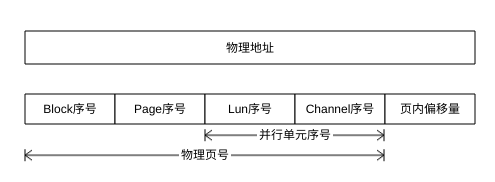
\includegraphics[width=0.8\textwidth]{paddrmap.png}
    \caption{开放通道SSD的物理地址与内部结构的对应关系}
    \label{fig:res_paddrmap}
\end{figure}
开放通道SSD按照如图\ref{fig:res_paddrmap}方式将物理地址编号与内部结构进行对应。一个用整形数表示的物理地址PA,从低位到高位各取若干位作为业内偏移量offset,Channel序号C,Lun序号L,Page序号P,Block序号B,则PA指向的开放通道SSD内部具体位置即为:第C个Channel的第L个Lun的第B个Block的第P个Page中从Page起始位置算起的第offset个Byte。将Lun和Channel放在地址的低位可以使连续的地址被分配到不同的Lun和Channel上,有利于利用设备内部的并行性。

页映射使用图\ref{fig:res_paddrmap}中Block序号、Page序号、Lun序号和Channel序号拼接得到每个物理页的唯一ID——物理页号。由于Lun和Channel的操作均相互独立,二者都被视为并行单元,为了对并行单元统一编号,使用图\ref{fig:res_paddrmap}中Lun序号和Channel序号拼接得到唯一的并行单元序号。

\section{优化策略设计}
由于目前开放通道SSD上开源的闪存转换层pblk采用页映射和贪心垃圾回收方式,并通过在各个Channel和Lun轮转选择写入和擦除块的方式实现负载均衡,故首先使用上述方式实现一个基本的优化策略,而后分别在映射方式和垃圾回收方面加以改进,同时保持原有的负载均衡机制。

\subsection{页映射-贪心垃圾回收策略(PM\_GCL)}
\subsubsection{重要结构描述}

\begin{table}[htb]
    \centering
    \begin{minipage}[t]{0.8\linewidth}
    \caption{页映射-贪心垃圾回收策略(PM\_GCL)重要结构描述}
    \label{tab:imple_pmstruct}
      \begin{tabularx}{\linewidth}{lX}
        \toprule[1.5pt]
        {\heiti 结构名称} & {\heiti 作用} \\\midrule[1pt]
        vpg2ppg & 页映射表\\
        ppg2vpg & 逆页映射表\\
        blk\_list & 每个并行单元上的块分配管理结构\\
        empty\_blks & 当前并行单元上的空闲块队列\\
        active\_blk & 当前并行单元上的活跃写入块\\
        non\_empty\_blks & 当前并行单元上已写满的块队列\\
        next\_ch\_lun\_i & 记录上次进行空间管理操作的并行单元序号的后继\\
        \bottomrule[1.5pt]
    \end{tabularx}
\end{minipage}
\end{table}

表\ref{tab:imple_pmstruct}描述了页映射-贪心垃圾回收策略用到的重要结构。

vpg2ppg为页映射表,用于完成逻辑页到物理页的映射。页映射方式的好处是映射关系较为灵活,缺点是页映射表的占用空间较大:设每个表项占用空间为$T$Byte,设备每个页容量为$P$Byte,则映射表所需空间为设备总容量的$T/P$。取$T=8, P=32768$,则映射表体积为整个设备容量的$1/4096$。当设备容量为4TB时,映射表所需内存高达1GB。页映射的另一个缺点是对映射表的更新操作较频繁,在进行覆盖写或垃圾回收操作时,物理位置发生变化的每个页的映射表项都需要更新。
ppg2vpg为逆页映射表,记录了每个物理页对应的逻辑页,用于标记物理页的分配状态,同时用于在垃圾回收过程中快速确定需重新写入的脏页对应的逻辑页号从而修改映射关系。

blk\_list为每个并行单元上用于分配单元内部块空间的管理结构。SSD设备的每个Channel和Lun的操作互相独立,均可视为一个并行单元。该结构通过2个队列和1个活跃块指针完成块空间的分配。empty\_blks用于管理当前单元内尚未被写入的块(空闲块),当需要分配空间时该结构将从空闲块队列上取下一个块,并将其设置为活跃写入块active\_blk用于放置对该单元的所有写入请求。活跃写入块写满后会被加入non\_empty\_blks队列等待垃圾回收。

为了最大程度利用设备的并行性,需要尽量使连续的逻辑页被分配到不同并行单元上。next\_ch\_lun\_i用于记录上次进行空间管理操作使用的并行单元序号的后继,用于使写入在不同单元之间进行轮转。

\subsubsection{映射方式}
\label{ssc:mapping}
\begin{figure}[H]
    \centering
    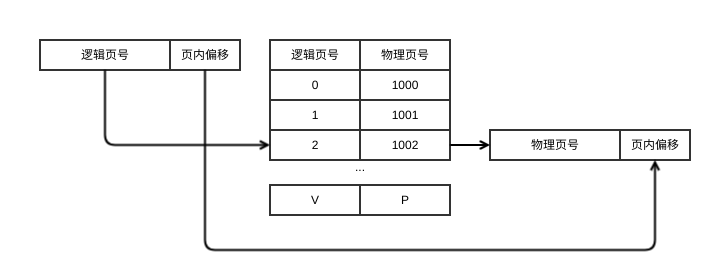
\includegraphics[width=0.8\textwidth]{page_mapping.png}
    \caption{页映射过程示意图}
    \label{fig:res_page_mapping}
\end{figure}

这一策略的映射方式使用页映射,映射过程如图\ref{fig:res_page_mapping}所示。逻辑页号由$\text{逻辑地址}/\text{页大小}$得到。物理页号由$\text{物理地址}/\text{页大小}$得到,对应图\ref{fig:res_paddrmap}中Block序号、Page序号、Lun序号和Channel序号共同组成的部分。对于传入的每个逻辑地址,策略通过查找页映射表将逻辑页号转换为物理页号,页内偏移量不进行改变,从而得到对应的物理地址。

对于写请求,策略总是需要为传入逻辑地址的逻辑页号分配新的物理页号:若当前逻辑页号尚未分配物理页号则显然需要;若已分配物理页号,则当前的写操作为覆盖写,需要将该物理页数据标记为无效,然后重新分配新的物理页存放覆盖写入的数据。分配新物理页号的过程如下:从next\_ch\_lun\_i开始遍历所有的并行单元,若遇到某个并行单元存在活跃写入块,或者不存在活跃写入块但存在空闲块则选择该单元进行空间分配。若所选单元没有活跃写入块则从空闲块队列中取出一个作为活跃写入块。若遍历所有并行单元后不存在符合条件的并行单元,则进行一次垃圾回收后重复遍历过程。遍历完成后,更新next\_ch\_lun\_i为当前选择单元的下一单元。最后,在所选的并行单元的活跃写入块中任意选择一个空闲页作为分配的新物理页,写入数据并更新页映射表和逆页映射表。

% 该过程中用到的主要接口如表\ref{tab:imple_pminf}:

\begin{table}[htb]
    \centering
    \begin{minipage}[t]{0.8\linewidth}
    \caption{页映射-贪心垃圾回收策略(PM\_GCL)映射过程主要接口}
    \label{tab:imple_pminf}
      \begin{tabularx}{\linewidth}{lX}
        \toprule[1.5pt]
        {\heiti 接口名称} & {\heiti 作用} \\\midrule[1pt]
        vpg2ppg(lm, vpg\_i) & 在映射表lm中查询,获取逻辑页号vpg\_i对应的物理页号\\
        ppg2vpg(lmr, ppg\_i) & 在映射表lmr中查询,获取物理页号ppg\_i对应的逻辑页号\\
        isalloc(lm, vpg\_i) & 查询逻辑页号vpg\_i是否已被分配物理页号\\
        allocate\_page(lm, vpg\_i) & 为逻辑页号vpg\_i分配物理页号,并维护映射表\\
        \bottomrule[1.5pt]
    \end{tabularx}
\end{minipage}
\end{table}

\subsubsection{垃圾回收}
垃圾回收过程中回收块的选择基于贪心策略:每次均选择所有已写满块中有效数据最少的一个块进行回收,在擦除的时间消耗一定时,贪心策略可以最小化重新写入脏页消耗的时间,同时最大化释放的空间。垃圾回收时机的选择遵循懒惰原则:当前写请求需要写入的数据量大于当前可用空闲页所能容纳的数据量时进行一次或多次垃圾回收,直到剩余空闲页能够容纳当前写入数据量为止。

垃圾回收的具体逻辑如下:首先从next\_ch\_lun\_i开始,遍历所有逻辑单元中的已写满的块队列,记录含脏页最少的块并选择为待回收块。遍历完成后更新next\_ch\_lun\_i为待回收块所在单元的后继单元。将待回收块内的所有脏页读入缓存并记录每个脏页所属的逻辑页号。将其移出该单元的已写满块队列,擦除该块,然后加入该单元的空闲块队列。对于读入的每个脏页,按照\ref{ssc:mapping}中的空间分配方式为其分配新的物理页,写入相应数据并更新映射表。由于被垃圾回收的任何块中脏页数量都小于该块的总页数,故每个脏页在原块被擦除成为空闲块后均能被分配新的物理页。

\subsubsection{负载均衡}
负载均衡主要通过以下2种机制实现:

物理页分配过程中,每次分配都会选择不同的并行单元上的活跃块空闲页,如此可以保证逻辑空间上连续的写入请求被均匀分布到不同的并行单元上,同时每个并行单元活跃块的选取遵循先进先出(FIFO)原则,刚刚被写满的活跃写入块只能加入写满块队列的尾部,等到其完成垃圾回收后又只能加入空闲块队列的尾部,在它第二次成为活跃写入块之前其他所有块都要完成一次擦除-写满的过程,因此不会出现同一个块被反复擦写而其他块不被访问的情况,故写负载在每个并行单元内也能够均匀分布到每个块上。

垃圾回收过程中,由于多个块同时具有最小脏页数量的情况时常出现,而垃圾回收算法总会选择其中第一个被访问的块,因此遍历时利用next\_ch\_lun\_i指针同样可以使得回收块的选择在不同并行单元上均匀分布。而物理页分配机制保证了每个单元中的块不会被短时间内多次写满,故擦除操作同样可以均匀分配到单元内的所有块上。


\subsection{页映射-连续空间垃圾回收策略(PM\_GCC)}
贪心垃圾回收需要为每个并行单元提供空间管理功能,结构略显复杂。一种可能的改进方式是模仿日志结构化文件系统\cite{rosenblum_design_1992}的做法改进空间分配和垃圾回收方法。

\subsubsection{重要结构描述}
\begin{table}[htb]
    \centering
    \begin{minipage}[t]{0.8\linewidth}
    \caption{页映射-连续空间垃圾回收策略(PM\_GCC)重要结构描述}
    \label{tab:imple_lsstruct}
      \begin{tabularx}{\linewidth}{lX}
        \toprule[1.5pt]
        {\heiti 结构名称} & {\heiti 作用} \\\midrule[1pt]
        vpg2ppg & 页映射表\\
        ppg2vpg & 逆页映射表\\
        used\_begin\_ppg & 已写入区的起始物理地址\\
        used\_end\_ppg & 已写入区的结束物理地址\\
        \bottomrule[1.5pt]
    \end{tabularx}
\end{minipage}
\end{table}
表\ref{tab:imple_lsstruct}描述了该策略用到的重要结构。与页映射-贪心垃圾回收策略相比,该策略取消了对每个并行单元的空间管理,代之以划分设备空间为2个物理地址上连续的空间——已写入区和空闲区的做法。策略通过维护已写入区的起始物理地址used\_begin\_ppg和结束物理地址used\_end\_ppg(同时分别为空闲区的结束物理地址和起始物理地址)即可实现该功能。

\subsubsection{映射方式}
该策略的映射方式同样采用页映射,其地址转换机制与图\ref{fig:res_page_mapping}相同,接口形式与表\ref{tab:imple_pminf}相同,这里不再赘述。

初始状态下设备全部空间为空闲区。每次分配新的物理页时,设备将当前已写入区所在的结束物理地址指向的物理页分配出去,同时将该物理地址数值增加一个页的大小。根据\ref{imple:paddrmap}中的对应规则,增加后的物理地址将指向下一个并行单元的相同位置。这样对每个页的写入能够被分配到不同的并行单元上。
\subsubsection{垃圾回收}
该策略垃圾回收时机的选择同样基于懒惰原则:当空闲区的容量小于当前写入量时进行垃圾回收。在单次写入量小于Block容量的情况下,一次垃圾回收往往涉及对整个设备上所有块的访问。

垃圾回收时需要遍历整个已写入区,读出脏页和所属逻辑地址,擦除完成后重新写入并更新页映射表。遍历时为了利用并行性,同样遵循并行单元->Page->Block的遍历顺序,因此对Block的遍历并非逐个完成,而是一次完成并行单元数个Block的遍历,这要求用于存放脏页的缓存大小至少为并行单元数个Block大小。
\subsubsection{负载均衡}
从该策略的物理页分配方式可知,该策略将所有写操作均转换为对设备所有物理页的顺序写操作,因此写操作可以在所有页上均衡分布;在懒惰原则下和单次写入量不超过Block容量的情况下,一次垃圾回收会对设备的所有块进行擦除操作,故擦除操作同样能够均匀分布在所有块上。

\subsection{超级块映射-贪心垃圾回收方式(SBM\_GCL)}
另一种改进思路是增大映射的粒度。根据之前对高性能应用负载的分析,其IO Trace中存在大量的按页甚至按块对齐的覆盖写,因此在覆盖写过程中很可能出现整块的数据被标记为无效、需要回收的块完全不含脏页的情况。在这种情况下,逻辑地址与物理地址之间的映射往往是以块为单位进行的,采用粒度为块的映射完全可以在达到与页映射相同效果的同时大幅减少映射表占用空间和修改开销。
基于这一想法本文提出了超级块映射的改进方法,即将映射粒度从页增大到由一个或者多个块组成的超级块。
\subsubsection{重要结构描述}
\begin{table}[htb]
    \centering
    \begin{minipage}[t]{0.8\linewidth}
    \caption{超级块映射-贪心垃圾回收策略(SBM\_GCL)重要结构描述}
    \label{tab:imple_sbmstruct}
      \begin{tabularx}{\linewidth}{lX}
        \toprule[1.5pt]
        {\heiti 结构名称} & {\heiti 作用} \\\midrule[1pt]
        PN & 每个超级块包含的并行单元数\\
        BN & 每个超级块的每个并行单元包含的块数\\
        vsblk2psblk & 超级块映射表\\
        psblk2vsblk & 逆超级块映射表\\
        sblk\_list & 每个超并行单元上的超级块分配管理结构\\
        empty\_sblks & 当前超并行单元上的空闲超级块队列\\
        non\_empty\_sblks & 当前超并行单元上写入过的超级块队列\\
        next\_ch\_lun\_i & 记录上次进行空间管理操作的并行单元序号的后继\\
        \bottomrule[1.5pt]
    \end{tabularx}
\end{minipage}
\end{table}
表\ref{tab:imple_sbmstruct}描述了超级块映射-贪心垃圾回收策略所用的重要数据结构。

参数PN和BN定义了超级块的大小,每个超级块含有PN个并行单元,每个并行单元含有BN个块,故一个超级块含有$\mathrm{PN}\times \mathrm{BN}$个块。

该表中的其他结构与表\ref{tab:imple_pmstruct}中的结构大体相同,只不过将块替换为了超级块,同时由于每个超级块可能含有多个并行单元,故每PN个并行单元(称为一个超并行单元)分配一个超级块管理结构而不是每个并行单元都分配一个。一个区别是超级块映射中不需要为每个并行单元设置活跃写入块,non\_empty\_sblks队列不仅包含已被写满的超级块,也包含存在有效数据但尚未写满或者发生覆盖写的超级块。原因是在超级块映射下,一个超级块只要发生了覆盖写,即使该超级块尚未写满,其映射关系也需要更新,其中的所有数据被标记失效,所有脏页必须重新写入新超级块,随后该超级块中的脏页数量归零,随时可以进行垃圾回收。活跃写入块这种被写满后才可能被垃圾回收队列的机制在这里是不存在的。

\subsubsection{超级块地址结构}
超级块这一概念在开放通道SSD中并无实际物理结构对应,只是改变了块的组织方式,为了方便起见在此重新定义引入超级块后物理地址与开放通道SSD内部结构的对应关系。
\begin{figure}[H]
    \centering
    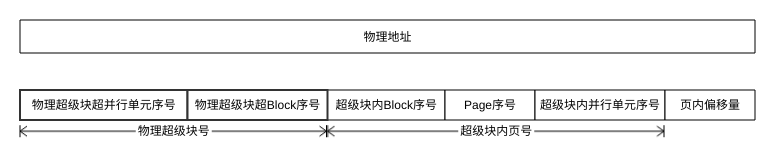
\includegraphics[width=0.8\textwidth]{sbaddrmapping.png}
    \caption{引入超级块概念后物理地址与开放通道SSD内部结构的对应关系}
    \label{fig:sbaddrmapping}
\end{figure}
对于一个Channel、Lun、Block、Page数分别为C、L、B、P的开放通道SSD,使用参数为PN、BN的超级块映射后物理地址与SSD内部结构的对应关系如图\ref{fig:sbaddrmapping}所示。一个物理地址PA可以从低位到高位依次划分为页内偏移量offset,超级块内并行单元序号inner\_pu,Page序号p,超级块内Block序号inner\_blk,物理超级块超Block序号outer\_blk,物理超级块超并行单元序号outer\_pu。该物理地址指向的SSD内部位置可按表\ref{tab:imple_sbaddrmapping}计算。在这种对应方式下,相邻的物理地址会对应到同一个超级块中,而在遍历同一个超级块内的地址时,遍历顺序仍然是按照并行单元->Page序号->Block序号进行的,即在同一个超级块内连续的物理地址仍然会分布在不同的并行单元上。
\begin{table}[htb]
    \centering
    \begin{minipage}[t]{0.8\linewidth}
    \caption{引入超级块概念后物理地址到开放通道SSD内部结构的转换方法}
    \label{tab:imple_sbaddrmapping}
      \begin{tabularx}{\linewidth}{lX}
        \toprule[1.5pt]
        {\heiti 参数} & {\heiti 值} \\\midrule[1pt]
        Channel 序号 & $(\mathrm{inner\_pu} + \mathrm{outer\_pu} \times (C \times L / PN))\mod C$\\
        Lun序号 & $(\mathrm{inner\_pu} + \mathrm{outer\_pu} \times (C \times L / PN)) \div C \mod L$\\
        Block序号 & $\mathrm{inner\_blk} + \mathrm{outer\_blk} \times (B / BN)$\\
        Page序号 & p\\
        页内偏移量 & $\mathrm{offset}$\\
        \bottomrule[1.5pt]
    \end{tabularx}
\end{minipage}
\end{table}

\subsubsection{映射方式}
\label{sssc:sbmapping}
\begin{figure}[H]
    \centering
    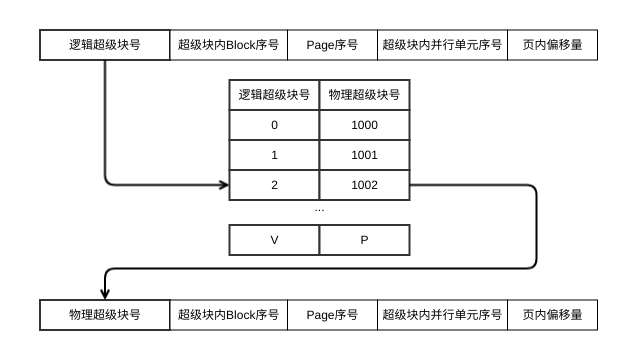
\includegraphics[width=0.8\textwidth]{sbmapping.png}
    \caption{超级块映射过程示意图}
    \label{fig:sbmapping}
\end{figure}
超级块映射与页映射的区别仅在于映射粒度,故图\ref{fig:sbmapping}中的地址映射过程与页映射类似。

对于写请求,该策略首先遍历写请求涉及到的逻辑页,尝试为每个逻辑页所在的逻辑超级块分配可用的物理超级块映射。若该逻辑超级块已经存在物理超级块映射,且逻辑页映射后的物理页可直接写入,则不改变映射关系;若该逻辑超级块不存在物理超级块映射或者存在映射但逻辑页对应的物理页为脏页,则需要为当前逻辑超级块分配新的物理超级块。分配流程与\ref{ssc:mapping}中分配物理页的过程类似:遍历所有超并行单元的分配管理结构,从空闲超级块队列中取出一个成员用于分配。若为写入脏页的情况,分配后除了写入当前写请求的数据和维护超级块映射表外,还要将原超级块的所有页标记为失效,并将其中未被覆盖写的脏页也写入新的超级块。

由于逻辑超级块和物理超级块是一一对应的关系,在不存在映射而进行分配的情况下策略必然能找到一个空闲超级块。但在待写入页为脏页而进行分配的情况下有可能出现无空闲超级块可用的情况,这时的处理方法有两种:一种是在读出未被覆盖写的脏页后直接擦除当前超级块,然后就地写入要写的数据和脏页;另一种方式是尝试进行垃圾回收,若回收得到超级块则继续按照分配成功的情况处理,若失败再回到第一种做法就地写入。第一种做法的优势是无需修改映射表,但由于映射表得不到更新,被擦除超级块的选择将完全取决于写请求访问的逻辑地址;第二种做法则更有利于负载均衡。

\subsubsection{垃圾回收}
由于引入超级块概念后物理地址与开放通道SSD内部结构的对应关系发生变化,连续空间垃圾回收方式中的已写入区和空闲区在引入超级块的对应方式下不再是物理地址上连续的区域,故采用超级块映射的优化策略无法使用连续空间垃圾回收,仍然采用基本优化策略的贪心垃圾回收方式。

垃圾回收的逻辑与页映射-贪心垃圾回收策略基本一致,区别仅在于将回收单位由块换成了超级块。一个简化的地方是由于超级块映射中需要回收的超级块内不存在脏页,故选择待回收超级块时可以直接选择脏页数为0的超级块而无需遍历所有待回收超级块获取脏页数量的最小值。

\subsubsection{负载均衡}
在贪心垃圾回收策略下,本优化策略具有与页映射-贪心垃圾回收策略相同的机制保证负载均衡。此外,\ref{sssc:sbmapping}中提到在写入页为脏页需要进行超级块分配但无空闲块可用时,先尝试垃圾回收后分配新超级块的方式与就地写入相比更有利于负载均衡,原因是该方式能够保持映射表的更新,使得相同的逻辑超级块地址多次访问时都能对应到不同的物理超级块地址,从而实现负载均衡。

% \section{映射方式}
% \subsection{直接地址映射}
% %直接地址映射即不进行任何形式的逻辑地址到物理地址的转换,这一策略最为简单,但不适用于SSD设备。原因是SSD设备的写入以Page为单位,而擦除以Block为单位,且被写入后的页只有在所在块被擦除后才能重新写入。当负载中存在大量的覆盖写时,

% \subsection{页映射}

% \subsection{超级块映射}

% \section{垃圾回收策略}
% \subsection{基于贪心原则的垃圾回收}
% \subsection{连续空间上的垃圾回收}

% \section{负载均衡}

\section{本章小结}
本章首先根据开放通道SSD访问特点确定了优化策略的实现层次,然后使用目前已有的开源闪存转换层pblk采用的地址映射、垃圾回收和负载均衡策略实现了最基本的优化策略。随后本章分别从垃圾回收算法和地址映射粒度两方面对基本策略尝试进行了改进,同时注意保持基本策略能够实现负载均衡的特点。
\chapter{实验结果与分析}
\label{cha:res}

实验将抓取的高性能应用的IO Trace通过映射和垃圾回收机制转换为对开放通道SSD内部结构操作,并使用liblightnvm对其进行直接读写,最后通过吞吐量、映射表修改次数、擦除次数和写放大系数等性能指标评价优化方法的优劣。此外,实验还研究了不同优化方法下剩余空间大小对IO性能的影响,以及超级块方法中超级块参数的影响。

\section{实验环境}
由于硬件条件限制,本章中所有实验均在开放通道SSD的模拟器上进行。因此,下文的"硬件环境"包括运行模拟器的设备的硬件环境,模拟器以及模拟出的开放通道SSD的基本参数。下文的"软件环境"包括模拟器使用的Linux内核版本与相关用户态库的信息。
\subsection{硬件环境}
实验使用一台Linux服务器运行模拟器,服务器的CPU为Intel(R) Xeon(R) CPU E5-2620 v2 @ 2.10GHz,内存大小16GB。模拟器使用https://github.com/DFC-OpenSource/qemu-ox 提供的支持模拟开放通道SSD的qemu虚拟机。除特殊说明外,实验使用的模拟开放通道SSD设备基本信息如下表:
\begin{table}[htb]
    \centering
    \begin{minipage}[t]{0.8\linewidth}
    \caption[开放通道SSD的基本信息]{开放通道SSD的基本信息}
    \label{tab:res_ocssd_geo}
      \begin{tabularx}{\linewidth}{cY}
        \toprule[1.5pt]
        {\heiti 参数名} & {\heiti 数值} \\\midrule[1pt]
        Channel数量 & 8\\
        每个Channel的Lun数量 & 4\\
        每个Lun的Block数量 & 64\\
        每个Block的Page数量 & 8\\
        每个Page的Sector数量 & 4\\
        Plane数量 & 2\\
        每个Sector能够容纳的数据量 & 4096 Byte\\
        每个Page能够容纳的数据量 & 32768 Byte\\ 
        \bottomrule[1.5pt]
    \end{tabularx}
\end{minipage}
\end{table}
\subsection{软件环境}
模拟器运行的Linux内核版本为4.17.0,编译时打开了CONFIG\_BLK\_DEV\_NVME,CONFIG\_NVM,CONFIG\_NVM\_DEBUG,CONFIG\_NVM\_PBLK选项以提供对开放通道SSD的驱动支持。实验使用的用于直接操作开放通道SSD设备的用户态库liglightnvm版本为master@ba201ca。

\section{IO吞吐量}
图\ref{fig:res_iototal}和表\ref{tab:res_iototal}展示了不同优化方法重放高性能应用的IO Trace时的IO吞吐量。可以发现,在重放LAMMPS和MACDRP两种应用的Trace时,与页映射-贪心垃圾回收方法相比,页映射-连续空间垃圾回收的IO吞吐量显著偏低,而超级块映射-贪心垃圾回收的方法IO吞吐量与之相接近。
\begin{figure}[H]
    \centering
    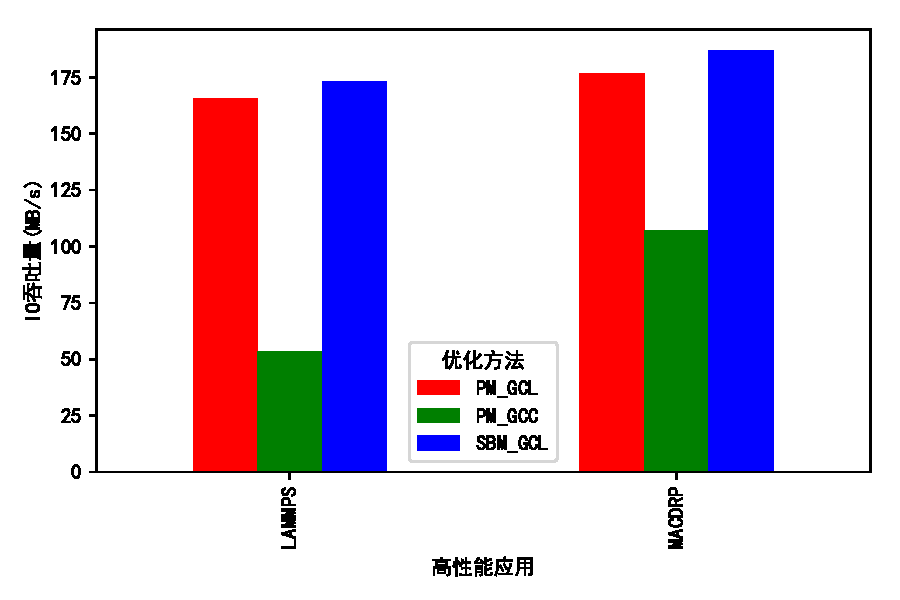
\includegraphics[width=0.8\textwidth]{iothroughput.pdf}
    \caption{不同优化方法的IO吞吐量}
    \label{fig:res_iototal}
\end{figure}

\begin{table}[htbb]
    \centering
    \begin{minipage}[t]{0.8\linewidth}
    \caption[不同优化方法的IO吞吐量(MB/s)]{不同优化方法的IO吞吐量(MB/s)}
    \label{tab:res_iototal}
    \begin{tabularx}{\linewidth}{cYYY}
        \toprule[1.5pt]
        \multirow{2}{*}{\heiti{高性能应用}} & \multicolumn{3}{c}{\heiti{优化方法}}  \\ \cmidrule(l){2-4} 
                     & PM\_GCL & PM\_GCC & SBM\_GCL \\ \midrule[1pt]
                     LAMMPS &65.448&53.217    & \textbf{173.116}    \\
                     MACDRP    & 176.768 &107.184    & \textbf{186.747}    \\ \bottomrule[1.5pt]
        \end{tabularx}
    \end{minipage}
\end{table}

为了更细致地刻画几种方法在IO吞吐量上的表现,以下从平均IO吞吐量在重放过程中的变化和单次IO吞吐量的分布来分析不同方法下的IO过程。
图\ref{fig:res_ioavg}反映了重放过程中平均IO吞吐量随IO请求总量的变化过程。
三种方法在早期均倾向于占据未分配的空间进行写入,当SSD上几乎所有空间均无法写入时开始进行垃圾回收,平均IO吞吐量开始下降并最终稳定到某个水平。对于页映射-贪心垃圾回收方法和超级块映射-贪心垃圾回收方法,二者每次进行垃圾回收均只需要回收一个块或者数个块的空间,且单次回收空间量的上限被本次IO的写入量所限制,故每次垃圾回收需要重新写入的脏页数量和需要擦除的块数量均相对较小。在这种机制下SSD上可直接写入的空间会长期维持在较低水平,每次写入均需进行小规模的垃圾回收,平均IO吞吐量受单次IO的影响较小。对于页映射-连续空间垃圾回收方法,由于空闲区域写满后需要在全盘范围内进行一次垃圾回收,需要擦除的块和重写的脏页遍布整个SSD,因此若当前IO无需进行垃圾回收则能够以顺序写的方式保持较高速率写入,若需要进行垃圾回收则要等待较长时间导致平均IO吞吐量突然下降。
连续空间垃圾回收每次均需要将当前有效数据重新写入,而贪心垃圾回收则未必。故连续空间垃圾回收的总成本更高,平均IO吞吐量更低,且在写入有效数据更多的LAMMPS的Trace上表现更差;而贪心垃圾回收的表现不受Trace写入的有效数据量影响。

\begin{figure}[H]
    \centering
    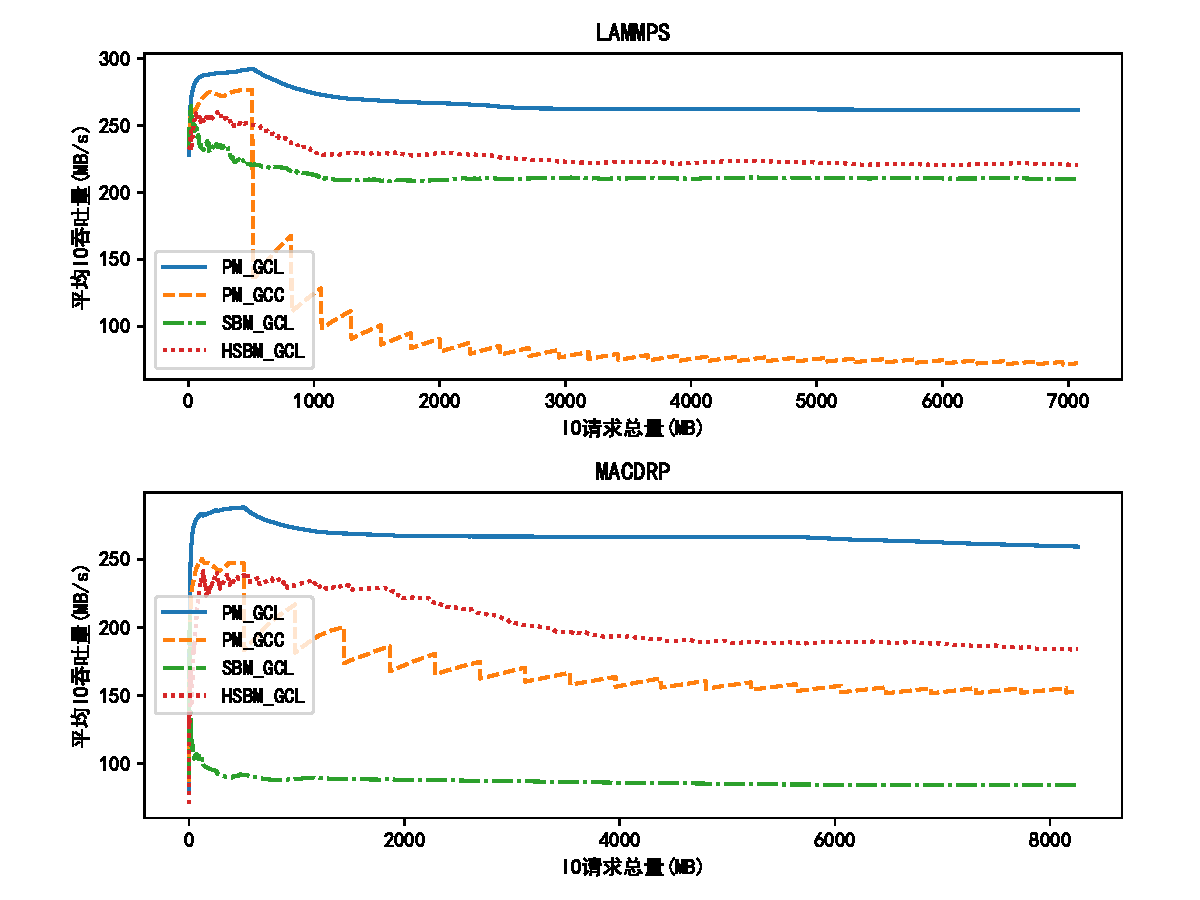
\includegraphics[width=0.8\textwidth]{avgiothp.pdf}
    \caption{平均IO吞吐量在重放过程中随IO请求总量的变化}
    \label{fig:res_ioavg}
\end{figure}

图\ref{fig:res_ioingle}按照IO请求发出的先后顺序绘制了每次IO的吞吐量。两种使用贪心垃圾回收策略的方法的单次IO吞吐量分布类似。连续空间垃圾回收方法尽管有大量写请求均能按照连续写速率(约300MB/s)写入,但每次发生垃圾回收时需要的开销过大,导致发生垃圾回收的写请求吞吐量接近0,整体吞吐量表现反而不如贪心垃圾回收方法。

\begin{figure}[H]
    \centering
    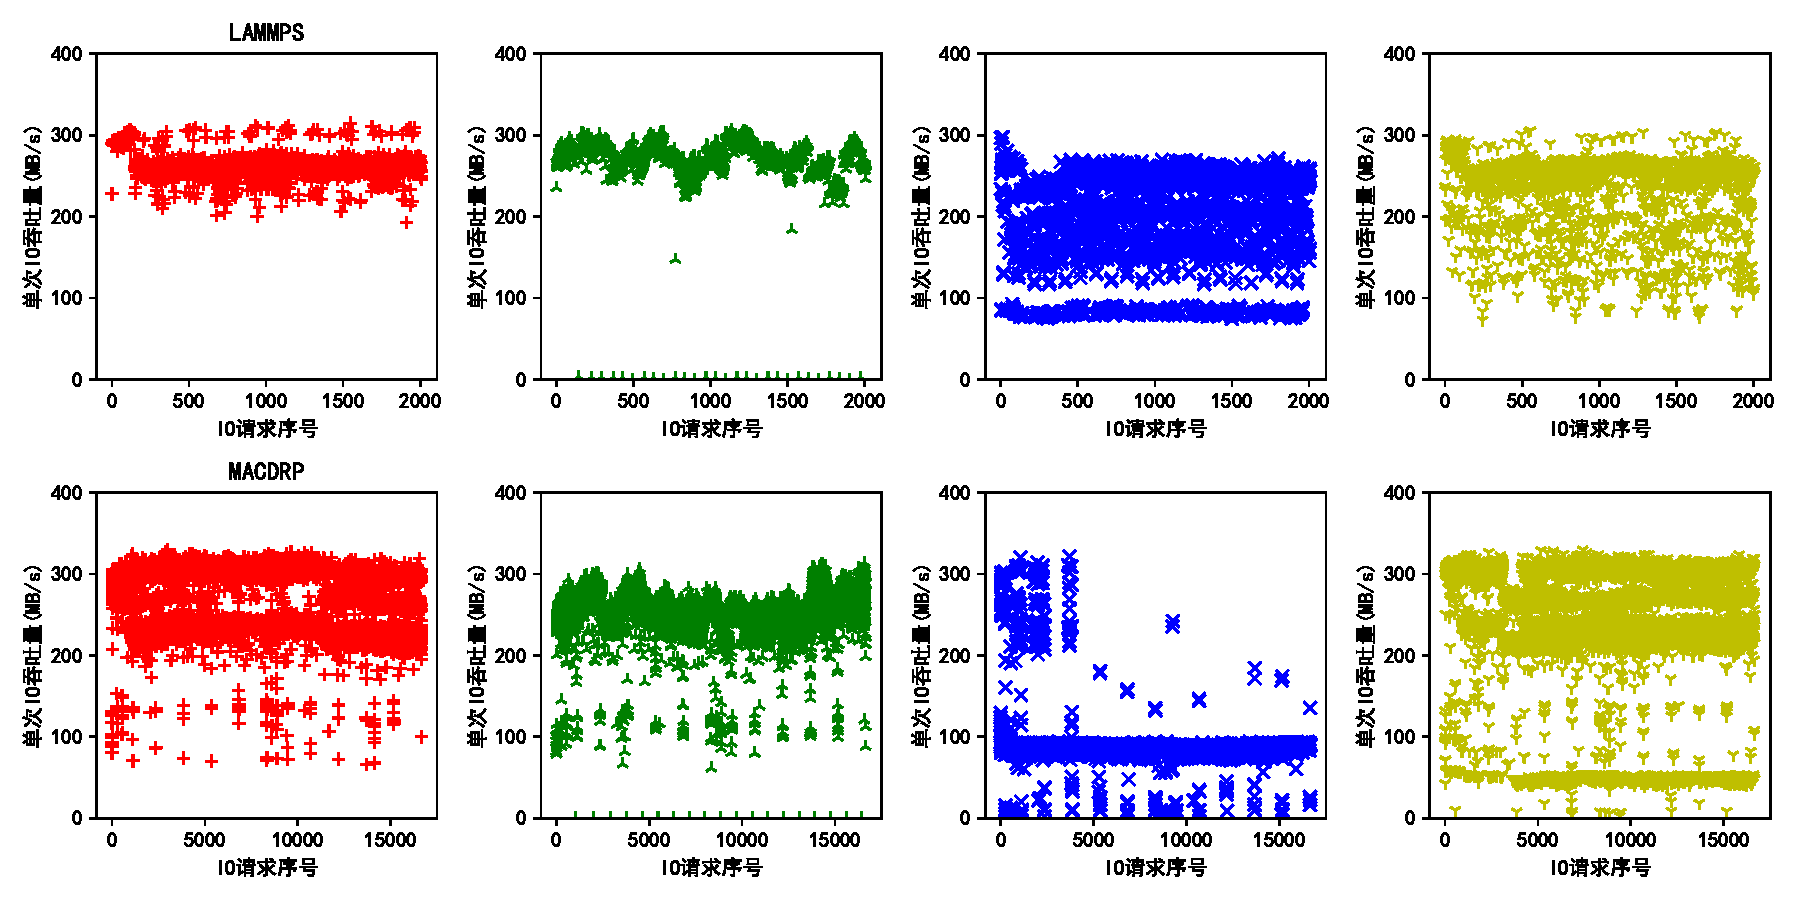
\includegraphics[width=0.8\textwidth]{singleiothp.pdf}
    \caption[不同优化方法在重放过程中的单次IO吞吐量]{不同优化方法在重放过程中的单次IO吞吐量,红色、绿色、蓝色分别代表页映射-贪心垃圾回收方法、页映射-连续空间垃圾回收方法和超级块映射-贪心垃圾回收方法}
    \label{fig:res_ioingle}
\end{figure}

\section{映射表开销}

超级块映射方法与页映射方法相比,其显著优势在于映射表占用空间更小,且维护映射表需要的成本更低。在映射表每个表项使用64位整形数存储对应的物理地址,占用空间为8Byte的条件下,对于实验用表\ref{tab:res_ocssd_geo}所示设备,页映射需要的映射表空间为$8\times 4\times 64\times 8\times 8\mathrm{Byte}=128\mathrm{KB}$,占设备全部可用空间的$1/4096$。而使用包含一个块的超级块映射,映射表所需空间为$8\times 4\times 64\times 8\mathrm{Byte}=16\mathrm{KB}$,占比仅为$1/32768$。由于超级块映射的表项更少,维护起来也更加简单。

\begin{figure}[H]
    \centering
    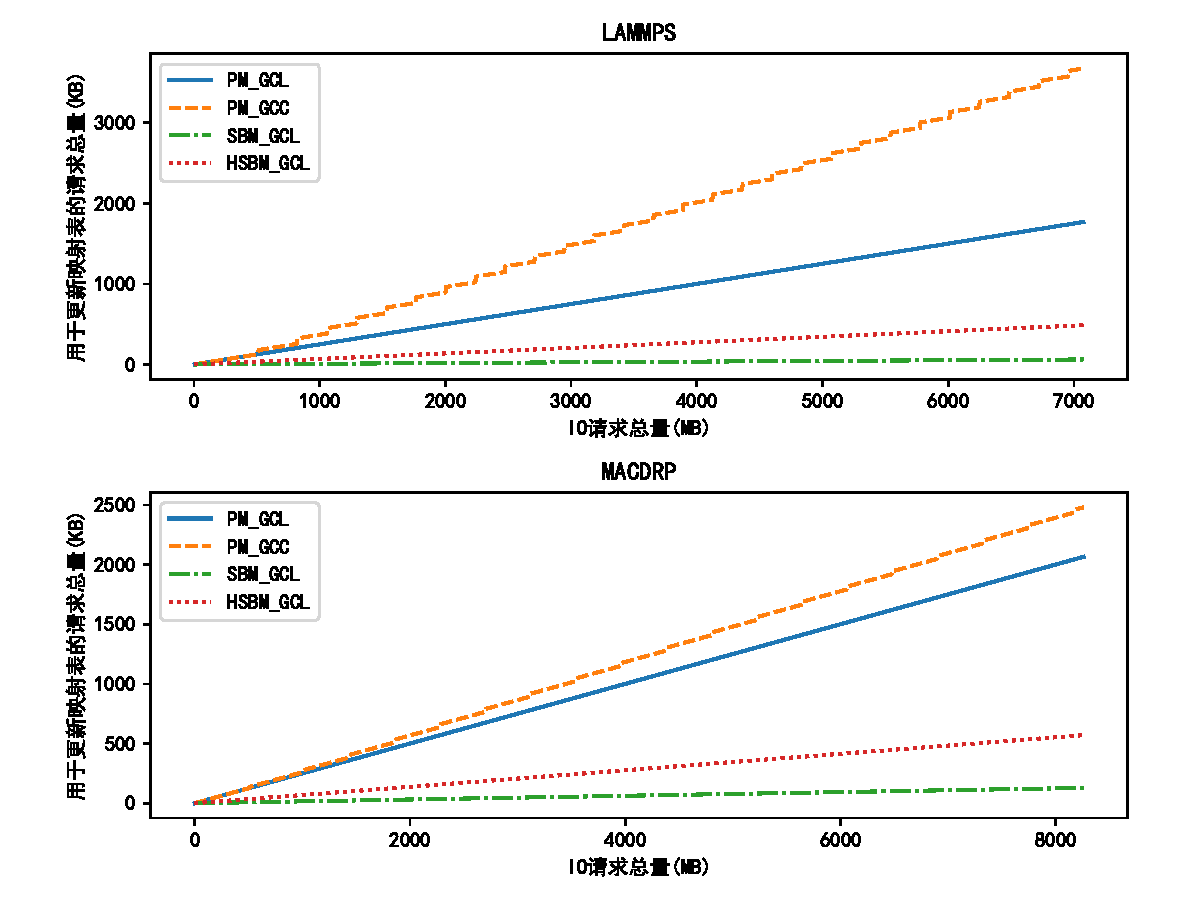
\includegraphics[width=0.8\textwidth]{mapupdateio.pdf}
    \caption{用于更新映射表的请求总量在重放过程中随IO请求总量的变化}
    \label{fig:res_mapupdate}
\end{figure}

如图\ref{fig:res_mapupdate},在LAMMPS负载下,页映射-贪心垃圾回收方法和页映射-连续空间垃圾回收方法每完成7G的IO写请求分别需要传输1768KB和3805KB的数据用于映射表更新,而超级块映射方法仅需要221KB;在MACDRP负载下,这一维护成本对于两种页映射方法分别为每8GB 2065KB和2477KB,对于超级块映射方法则仅为每8GB 259KB。

\section{擦除次数与写放大系数}

在设备自身的读写性能一定的情况下,映射算法和垃圾回收算法造成的擦除与写放大是影响整体吞吐量的最主要因素。这里以IO请求总量为变量,分析重放过程中擦除次数与写放大系数的变化。这里擦除次数定义为从重放开始擦除的Block总数,写放大系数定义为$\dfrac{\text{向设备写入的总数据量}}{\text{完成的写请求总数据量}}$。

\begin{figure}[H]
    \centering
    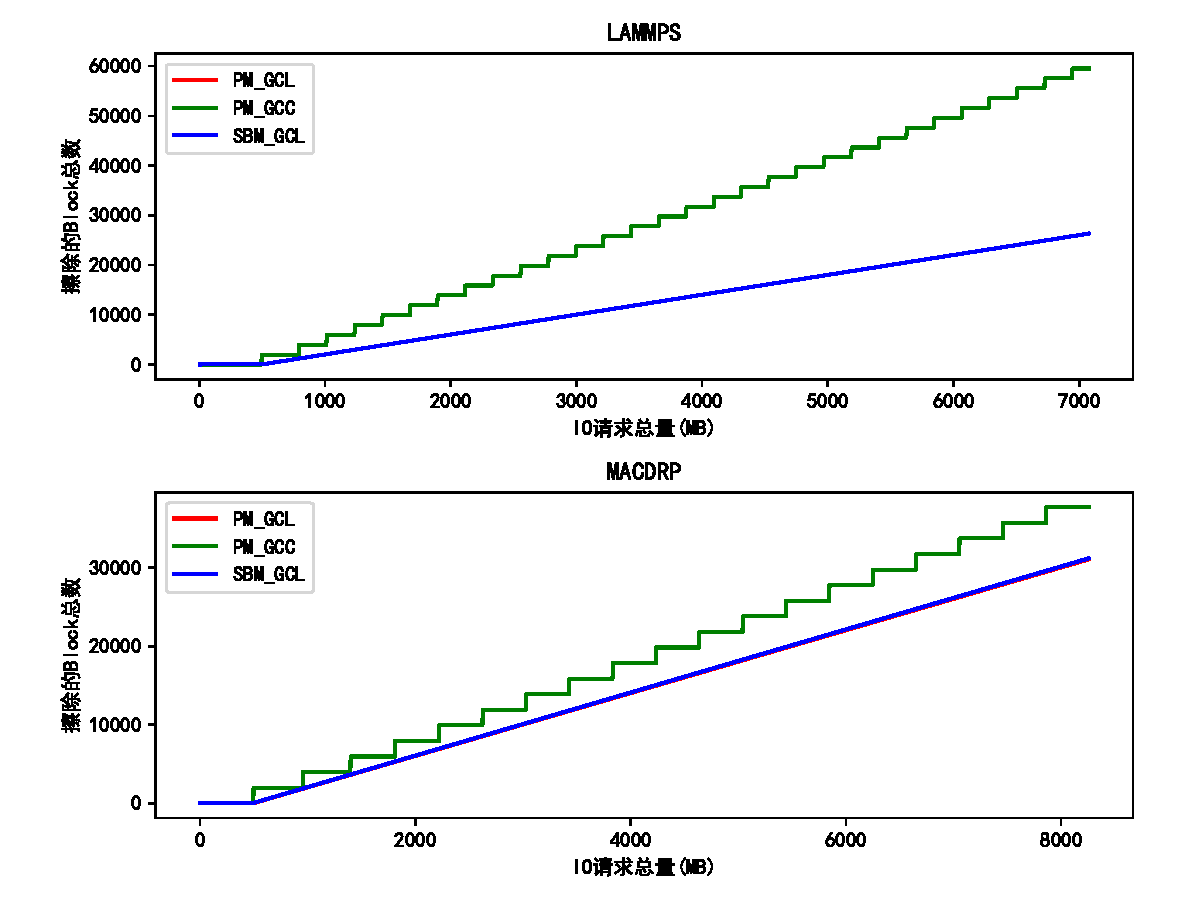
\includegraphics[width=0.8\textwidth]{eraseblk.pdf}
    \caption{擦除的Block数在重放过程中随IO请求总量的变化}
    \label{fig:res_erasecount}
\end{figure}

如图\ref{fig:res_erasecount},页映射-贪心垃圾回收方法和超级块映射-贪心垃圾回收方法的擦除次数与IO请求总量的关系几乎完全相同且近似线性变化。这是因为两种方法每次进行垃圾回收需要擦除的块数均受到当前IO写入量的控制,两种高性能应用每次IO请求的写入量相对恒定,与方法本身无关;两种方法下设备可直接写入的空间稳定在较低水平,每次写入均需要进行小范围的垃圾回收。页映射-连续空间垃圾回收方法的擦除次数呈现阶梯状变化,且写入有效数据较多的LAMMPS应用下擦除次数变化的间隔更小,原因是该方法每次垃圾回收后会腾出设备上除已写入有效数据的所有空间用于写入,待这段空间写满后才会再次进行垃圾回收,故两次垃圾回收之间有较大间隔;写入的有效数据越多,腾出的空间越少,垃圾回收间隔越小。

\begin{figure}[H]
    \centering
    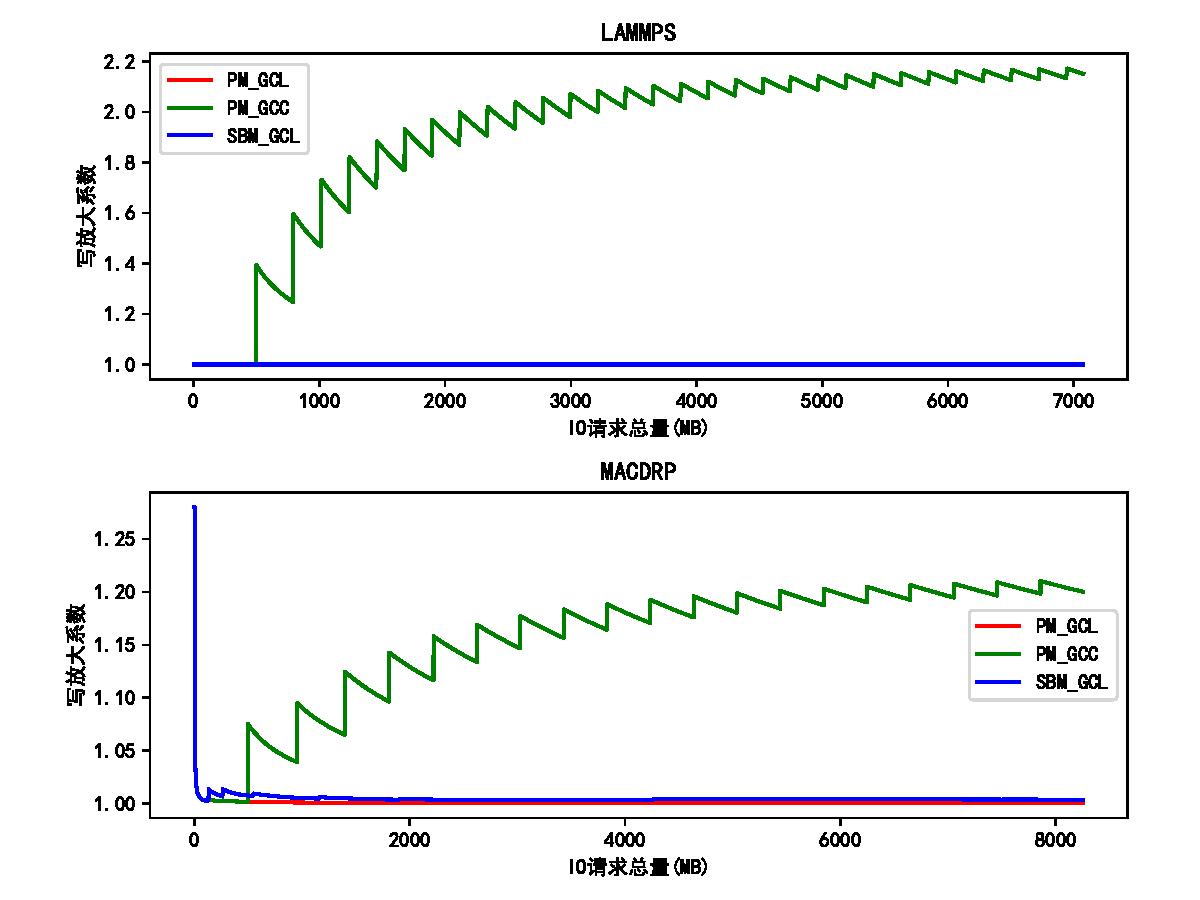
\includegraphics[width=0.8\textwidth]{writeampio.pdf}
    \caption{写放大系数在重放过程中随IO请求总量的变化}
    \label{fig:res_writeamp}
\end{figure}

如图\ref{fig:res_writeamp},两种贪心垃圾回收方法的写放大系数随着写入量增加很快稳定在1左右,而连续空间垃圾回收方法的写放大系数逐渐增加并维持在大于1的水平。两种应用的写请求起始位置绝大部分都按页对齐,一次连续写入的量大部分能覆盖一个或者多个Block,覆盖写的起始位置和大小与第一次写请求往往相同,因此每次覆盖写都会造成大量的整块Block中的数据无效。对于贪心垃圾回收,其只需要对相应块进行清除操作而无需重新写入大量脏页;对于连续空间垃圾回收,已写入的所有脏页均需要读出后重新写入,造成写放大系数偏高。

\section{负载均衡}

这里通过可视化设备上每个Page/Block执行写操作/擦除操作的次数比较不同方法的负载均衡情况。

\begin{figure}[H]
    \centering
    \subcaptionbox{重放LAMMPS时的负载分布}
      {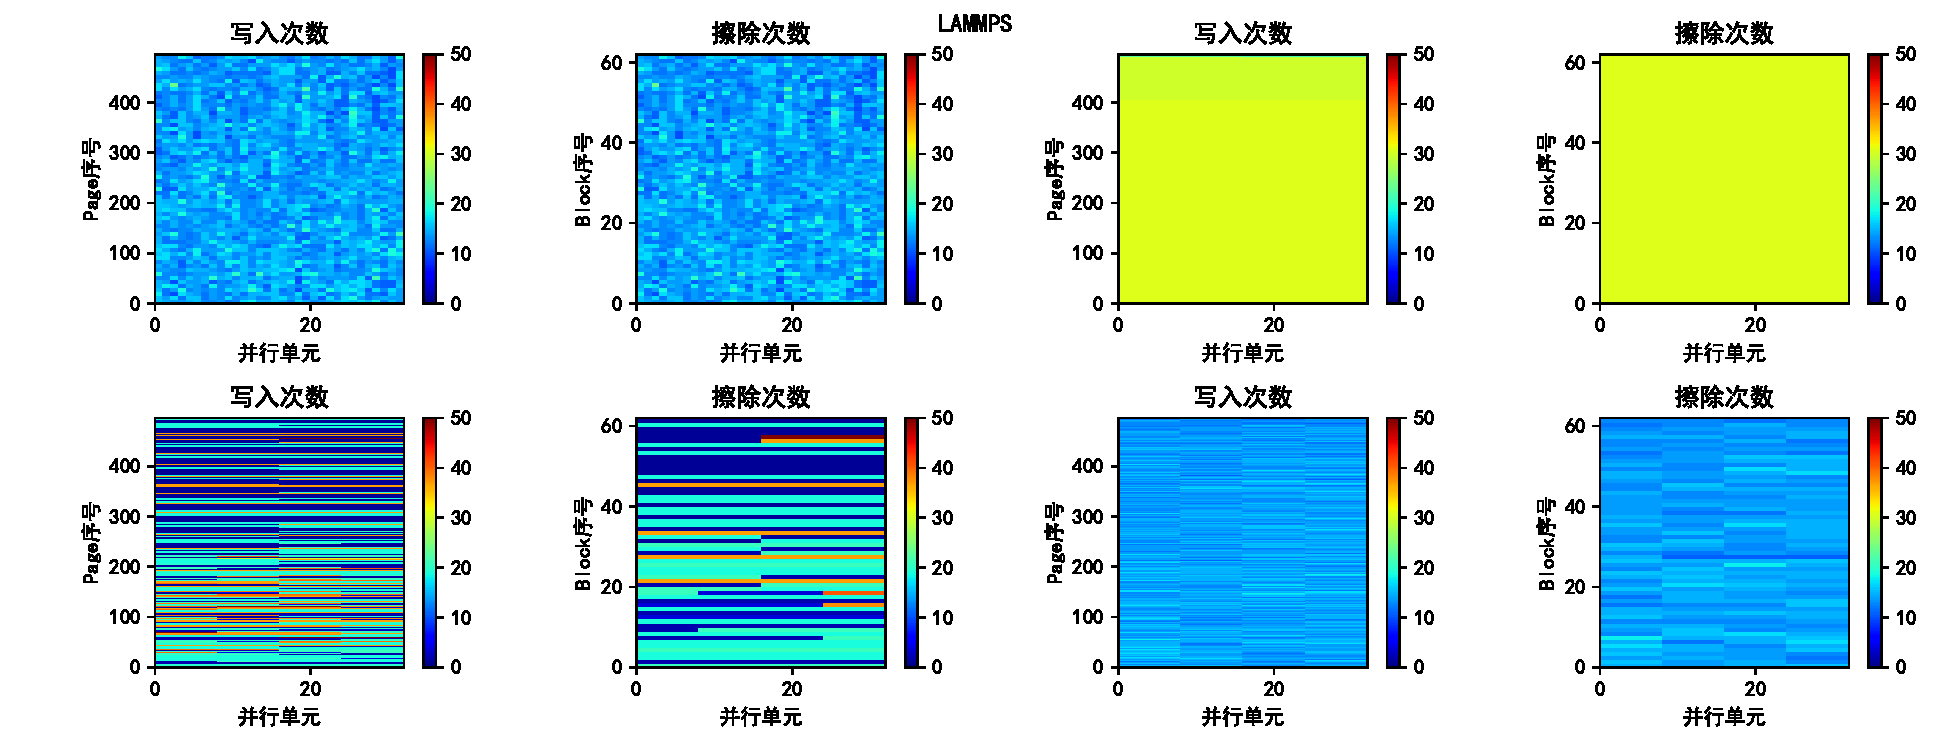
\includegraphics[width=0.8\textwidth]{heatmap_lammps.pdf}}
    \vspace{4em}
    \subcaptionbox{重放MACDRP时的负载分布}
        {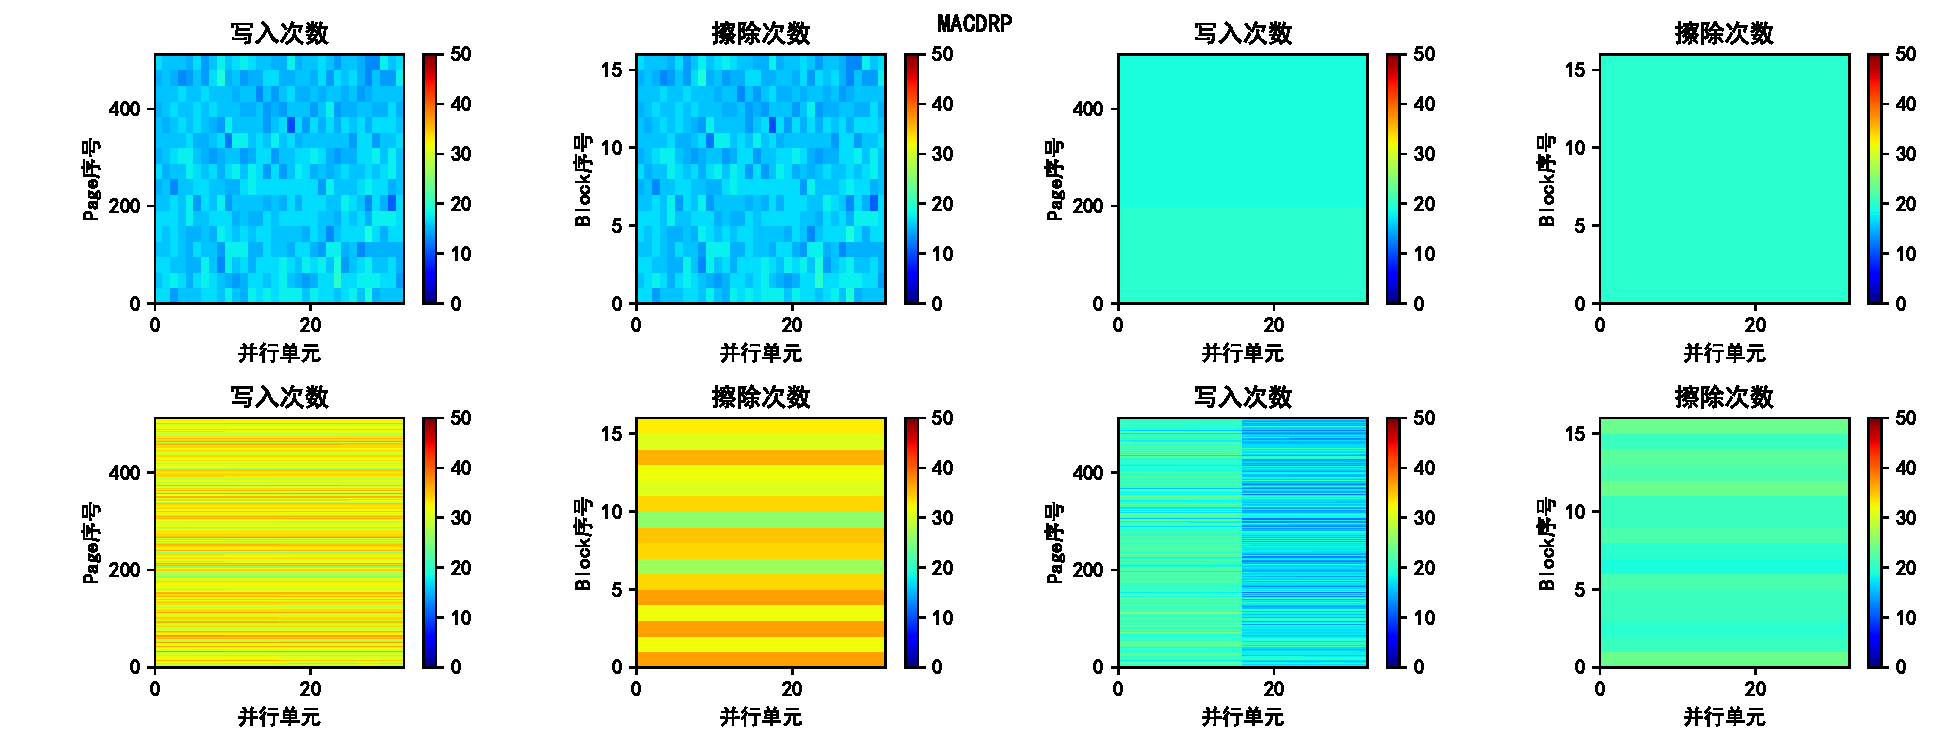
\includegraphics[width=0.8\textwidth]{heatmap_macdrp.pdf}}
    \caption[负载分布图]{负载分布图,每种应用的负载分布图的左上、右上、左下、右下各2张图分别代表页映射-贪心垃圾回收方法、页映射-连续空间垃圾回收方法、未改进负载均衡的超级块映射-贪心垃圾回收方法和改进后的该方法的写、擦除次数分布}
    \label{fig:res_heatmap}
\end{figure}

如图\ref{fig:res_heatmap},页映射-连续空间垃圾回收方法的负载均衡效果最好,所有位置的写入次数和擦除次数均几乎相同,原因是该方法在设备的几乎所有页被写入后才进行垃圾回收,而垃圾回收会对设备的所有块进行擦除,整个设备不断循环全部写入-全部擦除的过程。改进前的超级块映射-贪心垃圾回收负载均衡效果较差,因为在所有超级块均被写入并建立映射关系后,当前发生覆盖写的超级块中的脏页会在与写请求合并后就地重新写入擦除后的该块,映射关系不发生改变,导致被擦除的块的选择与写请求的起始位置有关。改进后的方法强制要求每次覆盖写选择另一位置的超级块写入,从而改善了负载均衡。

\section{设备容量的影响}

设备容量的大小可能对映射表维护和垃圾回收的开销产生影响。这里通过改变每个Lun含有的Block数量改变设备容量,使得设备容量分别为写入的有效数据量的2倍、4倍和8倍,观察这一变化对吞吐量、映射表修改次数、擦除次数和写放大系数等性能指标的影响。

\begin{figure}[H]
    \centering
    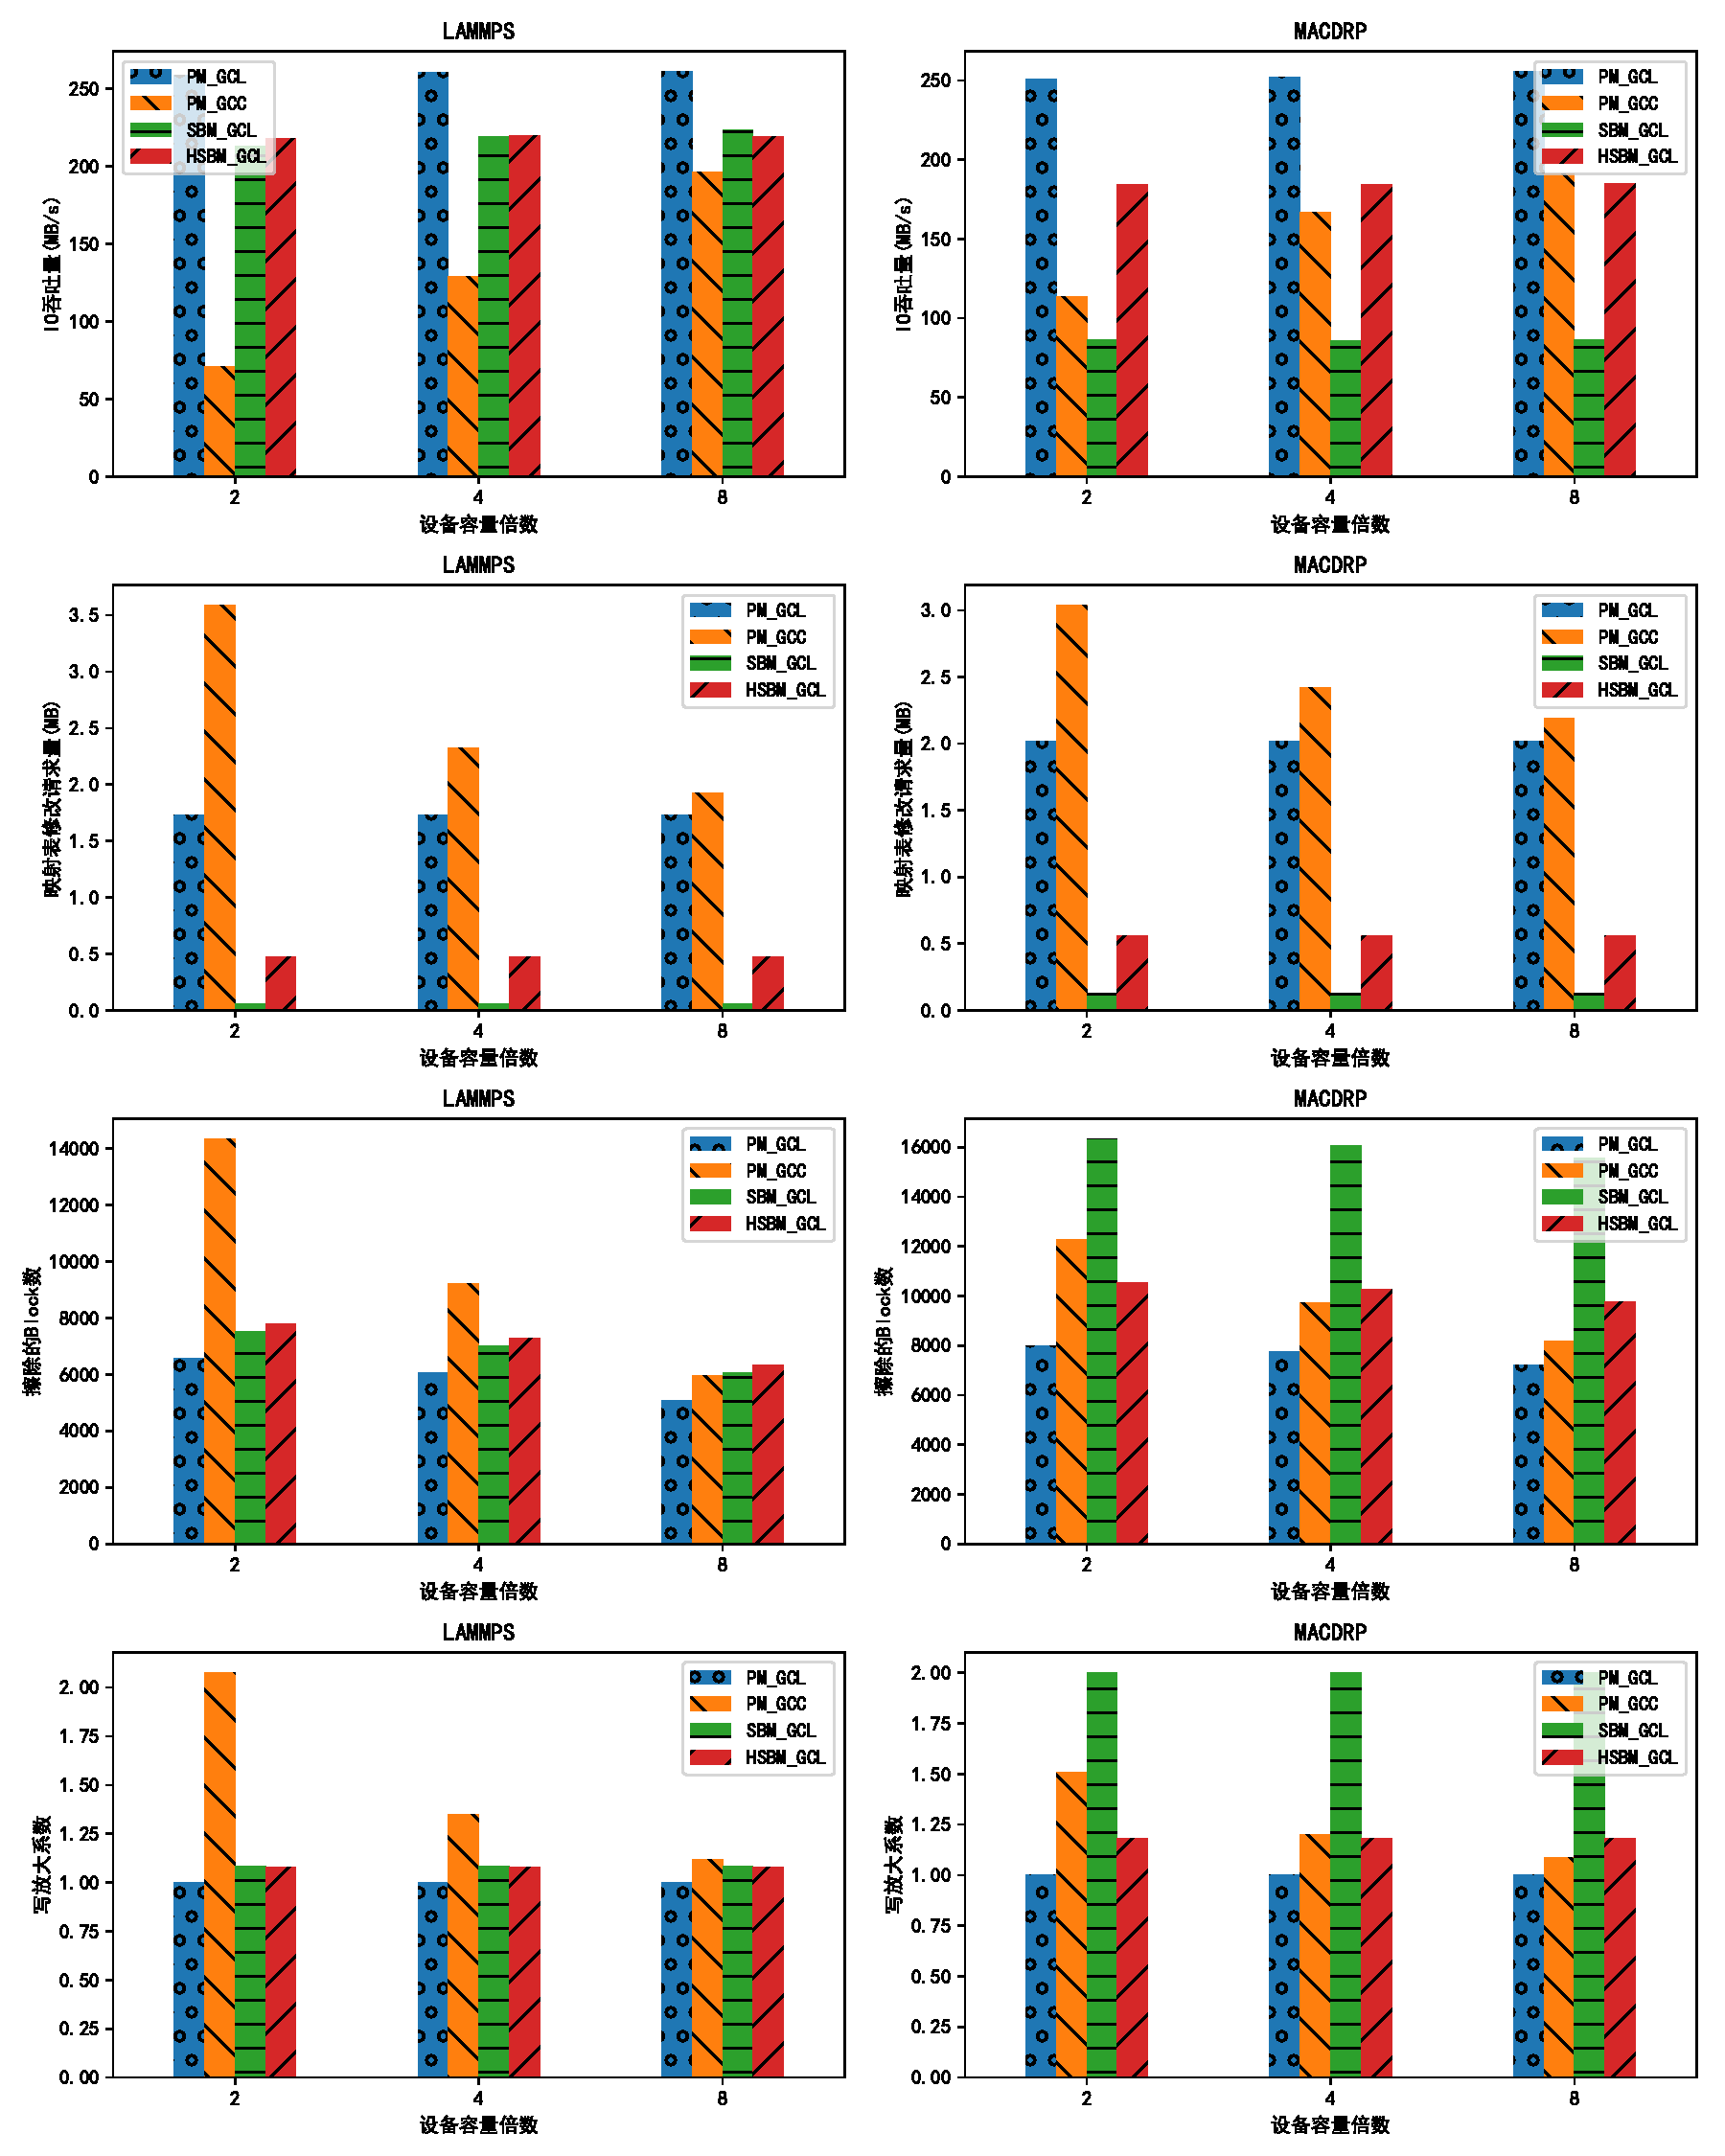
\includegraphics[width=0.8\textwidth]{disksize.pdf}
    \caption{设备容量对各项性能指标的影响}
    \label{fig:res_disksize}
\end{figure}

如图\ref{fig:res_disksize},页映射-贪心垃圾回收和超级块映射-贪心垃圾回收方法在设备容量增大时性能提高很小或基本不变,原因是设备容量增大只能延长两种方法第一次进行垃圾回收前连续写入的阶段,而这一阶段虽然无需进行垃圾回收,性能最好,但持续时间占整个重放过程的比例很低。达到稳定状态后两种方法都只在设备上维持很少的可用空间,开销与设备容量无关。对于页映射-连续空间垃圾回收方法,设备容量的增大增加了两次垃圾回收的间隔,尽管一次垃圾回收需要擦除的块数量更多,但垃圾回收次数减少和写放大系数降低带来的好处更大,故该方法在设备容量增大时性能提高较多。

\section{超级块大小的选择}

超级块映射涉及到设置为超级块设置合适的大小。较大的超级块能够显著减小映射表体积和维护成本,但发生覆盖写时需要擦除和重新写入的脏页数量也更多;较小的超级块则反之。这里通过调整超级块的大小为1、2、4、8个块,比较不同设置下超级块映射-贪心垃圾回收方法的性能指标。

\begin{figure}[H]
    \centering
    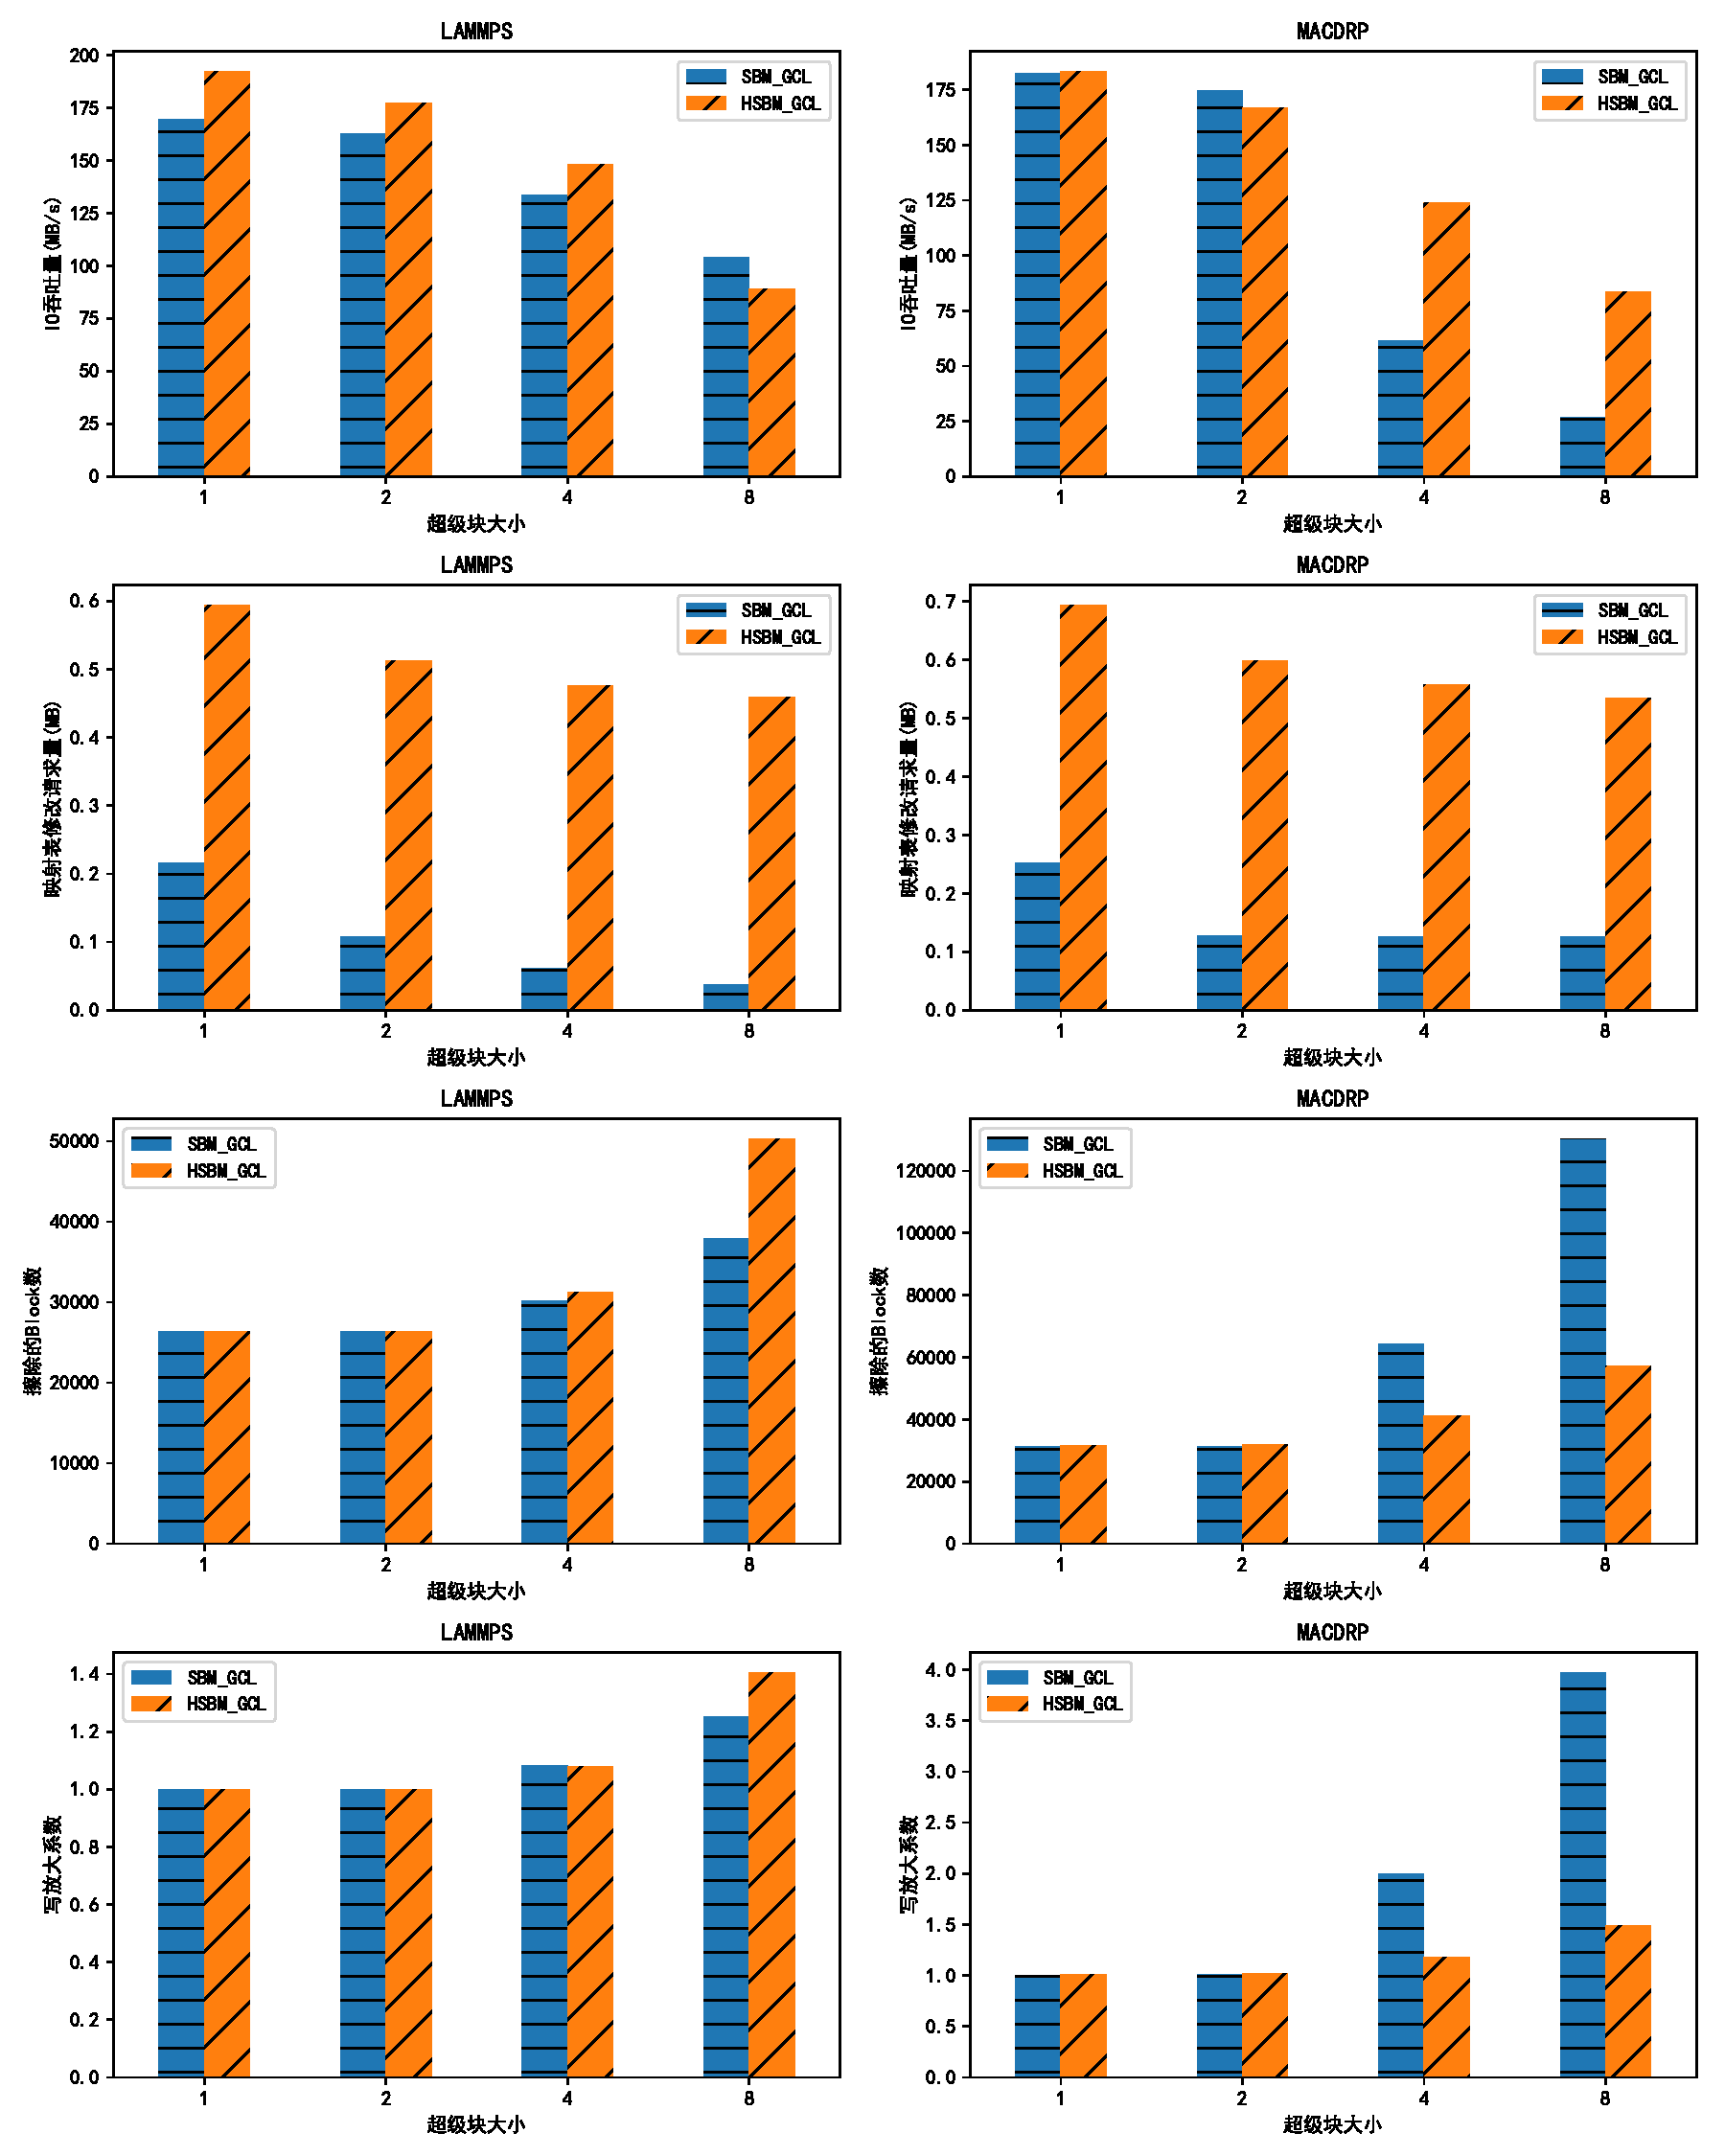
\includegraphics[width=0.8\textwidth]{sbsize.pdf}
    \caption{超级块大小对各项性能指标的影响}
    \label{fig:res_sbsize}
\end{figure}

如图\ref{fig:res_sbsize},超级块大小从1增加到2时,吞吐量有很小的下降,擦除次数和写放大系数几乎不改变,而映射表维护次数下降了接近50\%。超级块大小继续从2增加到4和8时,对于LAMMPS应用,吞吐量仍是小幅下降,擦除次数和写放大系数上升很小,映射表维护次数则继续随超级块大小翻倍而减半;对于MACDRP应用,吞吐量下降幅度较大,擦除次数和写放大系数大幅上升,映射表维护次数的变化与LAMMPS类似。其中的原因是LAMMPS一次连续写入的量往往在8个Block左右,因此增大超级块大小到8个Block后,每次连续写入后需要回收的块大部分依然不含脏页从而可以直接擦除,且相邻空间的写入仍然能映射到不同的超级块上;而MACDRP一次连续写入的数据量超过2个Block的比例较低,超级块大小超过2个Block后,每次连续写入的超级块很可能含有上次写入留下的脏页需要重新写入,造成较大的写放大系数;且相邻空间内的连续写入往往会映射到同一个超级块上,造成更多的映射冲突,进而引发更多的擦除和脏页重新写入。因此,对于高性能应用,超级块大小应尽量接近其占比最大的单次写入量大小但不能超过,以同时实现最小的映射表维护成本和覆盖写成本。

\section{本章小结}

本章使用吞吐量、映射表维护成本、擦除次数和写放大系数等指标评估了页映射-贪心垃圾回收、页映射-连续空间垃圾回收和超级块映射-贪心垃圾回收三种方法的性能,评估结果表明超级块映射-贪心垃圾回收方法能够在达到与页映射-贪心垃圾回收方法接近的吞吐量的同时,极大降低映射表体积和维护成本,证明页映射到超级块映射的改进适用于高性能应用在开放通道SSD上的IO优化;而连续空间垃圾回收与贪心垃圾回收相比劣势明显,不宜采用。之后本章讨论了设备容量对不同方法性能的影响,表明超级块映射-贪心垃圾回收方法与页映射-贪心垃圾回收方法一样受设备容量影响很小。最后本章讨论了超级块映射的重要参数——超级块大小的选取原则:应尽量接近所运行高性能应用占比最大的单次写入量大小但不能超过。
\chapter{结论与展望}
\label{cha:conclusion}
开放通道SSD因其能够将内部的结构暴露给外部程序从而提供更大的灵活性和更多的优化空间,得到了越来越广泛的应用,尤其是在数据库领域已经有了一些工作成果。但基于开放通道SSD优化高性能应用的工作目前还不多见。本文据此从两种高性能应用的负载特征分析入手,针对其特征实现了采用超级块映射和贪心垃圾回收方法的IO优化策略,相对于已有方法实现了接近的IO吞吐性能和更低的映射表维护开销。

本文利用高性能应用的IO负载中覆盖写比例较高的特点,判断其IO过程中会在SSD上产生大量不含任何脏页的无效数据块,从而将现有方法的映射粒度从页级别提升到超级块级别,在维持原有IO吞吐性能的同时降低了映射表的维护成本。本文同时尝试了模仿日志结构文件系统改进垃圾回收方式的做法,结果表明这一做法在垃圾回收时重新写入脏页的成本过高,写放大系数偏大,因而并不适用于本文所研究的高性能应用负载。

由于时间和精力所限,本文涉及的IO优化策略仅覆盖了地址映射、垃圾回收和负载均衡三方面的内容,实际系统中还可以通过写缓存、使用后台线程进行垃圾回收等方式进一步提高系统性能。这部分可以作为后续的研究内容。


%%% 其它部分
\backmatter

%% 本科生要这几个索引,研究生不要。选择性留下。
% 插图索引
\listoffigures
% 表格索引
\listoftables
% 公式索引
% \listofequations


%% 参考文献
% 注意:至少需要引用一篇参考文献,否则下面两行可能引起编译错误。
% 如果不需要参考文献,请将下面两行删除或注释掉。
% 数字式引用
\bibliographystyle{thuthesis-numeric}
% 作者-年份式引用
% \bibliographystyle{thuthesis-author-year}
\bibliography{ref/refs}


%% 致谢
% 如果使用声明扫描页,将可选参数指定为扫描后的 PDF 文件名,例如:
% \begin{acknowledgement}[scan-statement.pdf]
\begin{acknowledgement}
  衷心感谢导师舒继武教授和陆游游教授对本人的精心指导。他们的言传身教将使
  我终生受益。

  感谢季旭师兄帮助提供高性能应用的IO Trace,介绍应用背景和解释Trace文件含义。感谢李思阳师兄在实验初期提供各种负载模拟器资源和IO性能评测工具。感谢杨者同学在开放通道SSD模拟器使用和实验用服务器维护方面提供的帮助。

  感谢 \LaTeX 和 \thuthesis,帮我在排版论文时节省了不少时间。
\end{acknowledgement}


%% 附录
\begin{appendix}
\chapter{外文资料的调研阅读报告或书面翻译}

\title{从文件系统方面通过减少写入放大来延长基于闪存的存储的生命周期}

{\heiti 摘要:} 闪存由于其高性能,低能耗和低成本而作为用于企业和嵌入式系统的存储设备而广受欢迎。然而,闪存的耐用性问题仍然是一个挑战,随着存储密度随着多层单元(MLC)的采用而增加,这种问题正在变得越来越严重。之前的工作已经解决了损耗均衡和数据减少问题,但使用文件系统来提高闪存寿命的工作明显较少。传统文件系统中的一些常见机制(例如日志记录,元数据同步和页面对齐更新)会导致额外的写入操作并加剧闪存的磨损。这个问题被称为文件系统的写入放大。

为了减轻写入放大,我们提出了基于对象的闪存转换层设计(OFTL),其中的机制是与闪存协同设计的。通过利用页面元数据,OFTL能够实现索引元数据的惰性持久性,并在保持一致性的同时消除日志记录。粗粒度块状态维护减少了持久的空闲空间管理开销。借助字节单元访问接口,OFTL能够将小型更新与元数据进行压缩和共同定位,以进一步减少更新。实验表明,与最新页级别闪存转换层上的ext3,ext2和btrfs相比,基于OFTL的系统OFSS在SYNC模式下的写入放大率降低了47.4%〜89.4%,ASYNC模式下的写入放大率降低了19.8%〜64.0%。

\section{引言}
近年来,闪存技术有了很大的提高。随着主流设计从单层单元(SLC)转向多层/三层单元(MLC / TLC),基于闪存的存储正在见证容量的增加和每比特成本的降低,导致了在企业和嵌入式存储系统中应用的急速增长。但是,闪存密度的增加要求每个单元内有更精细的电压阶跃,这对泄漏和噪声干扰的耐受性较差。因此,闪存的可靠性和使用寿命大幅下降,产生了耐久问题[18,12,17]。

损耗均衡和数据缩减是延长闪存存储寿命的两种常用方法。通过磨损均衡,编程/擦除(P / E)操作倾向于分布在闪存块上,以使其均匀磨损[11,14]。数据缩减用于闪存转换层(FTL)和文件系统。 FTL引入了重复数据消除和压缩技术,以避免冗余数据的更新[15,33,34]。文件系统试图通过尾部打包[7]或数据压缩来减少更新[2,13]。但是,这些数据缩减技术在减少来自文件系统的写入放大方面效率低下,因为以下两个原因,从文件系统生成的元数据更新难以减少。一个是数据缩减不应损害文件系统机制。例如,在数据缩减中不应删除日志中的重复数据。另一个原因是大多数元数据出于一致性原因频繁同步,阻止了数据减少。

不幸的是,传统文件系统中的一些常见机制加剧了闪存写入放大。首先,通常用于保持更新原子化的日志记录加倍了写入大小,因为它将数据和元数据也复制到了日志。其次,元数据经常同步写入,以避免出现故障时的数据丢失。即使元数据占用的存储空间很小,频繁的写入操作也会产生巨大的写入流量,这对存储磨损产生巨大影响。第三,即使对于几个字节的更新,对存储设备的写入也是页对齐的。系统对来自应用程序的实际访问大小进行隐藏,因此更新强度被页面访问粒度放大。部分页面更新几乎总是需要读取 - 修改 - 写入。更糟糕的是,闪存页面大小的增加使得这个问题更加严重[17]。最后但并非最不重要的一点是,分层设计原则使得文件系统和设备彼此不透明,原因是窄块接口[35,29,28]。闪存存储上的文件系统机制无法解决耐久性问题,因此,使用这些机制,闪存会更快磨损。透明性还会阻止文件系统中的机制利用存储设备的特性。

事实上,闪存为更好的系统设计提供了机会。首先,每个页面都有一个页面元数据区域,也是OOB(带外)区域。保留空间可用于为索引元数据的惰性持久性或提供写入原子性的事务信息保留反向索引。其次,块被擦除后,闪存块的全部区域都变为干净状态。可以通过以擦除块(256 KB)为单位跟踪空闲空间而不是文件系统块(4 KB)来减少元数据开销。第三,与HDD(硬盘驱动器)相比,随机读取性能显著提高。部分页面更新可以被压缩,而不会引入显着的随机读取惩罚。如上所述,闪存特性可以用来缓解与系统协作时的耐久性问题。

我们提出了一种名为OFTL的基于对象的闪存转换层设计,将存储管理卸载到对象存储,并与闪存共同设计系统以减少写入放大。我们的贡献总结如下:

\begin{itemize}
\item 我们提出了OFTL,一个基于对象的闪存翻译层,以促进对数据的组织方式进行语义感知。
\item 为了降低索引元数据持久性和日志记录的成本,我们懒惰地刷新索引并通过在页面元数据中保留反向索引和事务信息来消除日志记录。
\item 我们还使用粗粒度块状态维护来跟踪页面状态,以降低可用空间管理的成本。
\item 使用OFTL中的字节单元接口,我们压缩部分页面更新并将它们与元数据共同定位以减少页面更新次数。
\item 我们实施基于OFTL的系统并在不同类型的工作负载下对其进行评估。结果显示,与现有文件系统相比,写入放大率显着降低。
\end{itemize}

本文的其余部分安排如下。第2部分给出了闪存和基于闪存的存储系统体系结构的背景。然后,我们在第3部分中介绍我们的OFTL设计,并在第4部分中与闪存共同设计系统机制。我们在第5部分中描述了实现,并在第6部分中评估了设计。相关工作在第7部分中介绍,第8节给出了结论。

\section{背景}
\subsection{闪存基础}
闪存以页为单位读取或写入,并以闪存块单位擦除。页面大小范围从512B到16KB [11,17]。每个Flash页面都有页面元数据,这些页面元数据与页面数据一起自动访问。通常,一个4KB页面有128B页面元数据[11]。闪存块由闪存页面组成,例如,一个256KB闪存块包含64页[11]。闪存块进一步排列在平面和通道中,以便在闪存驱动器内进行并行处理,称为内部并行。

与硬盘驱动器相比,闪存具有两个独特的特征,即不可覆盖属性和耐久性限制,这些都应该被文件系统设计考虑到。不可覆盖属性意味着被编程的页面不能被重新编程,直到它所在的闪存块被擦除。对编程页面的更新被重定向,以不可覆盖的方式清除页面,而编程页面无效以后再擦除。耐久性限制是每个存储器单元具有有限数量的P / E操作。存储器单元耗尽更多的P / E周期,导致寿命和可靠性的恶化。

\subsection{基于闪存的存储系统的体系结构}
闪存在嵌入式系统中广泛使用。在嵌入式系统中,闪存不支持块接口,并由文件系统直接管理,在该系统中实现映射,垃圾收集和耗损均衡。文件系统专用于闪存,称为闪存文件系统[10,32],如图1(a)所示。随着容量的增加和成本的降低,从笔记本电脑到企业服务器的计算机系统采用闪存设备作为HDD的替代品。 FTL在设备固件中实现以提供块接口,如图1(b)所示。

由于嵌入式FTL需要来自嵌入式处理器和大型DRAM的巨大计算能力来增加设备容量,因此FusionIO在称为VSL(虚拟存储层)的软件中实现了FTL,共享主机CPU周期和主存储器容量[4]。图1(c)显示了架构。基于软件的VSL为文件系统提供了优化的机会。在VSL上提出了DFS以利用VSL中的存储管理[20],并且使用日志结构的FTL从VSL中导出原子写入接口以向系统提供写入原子性[28]。

\begin{figure}[h]
  \centering
  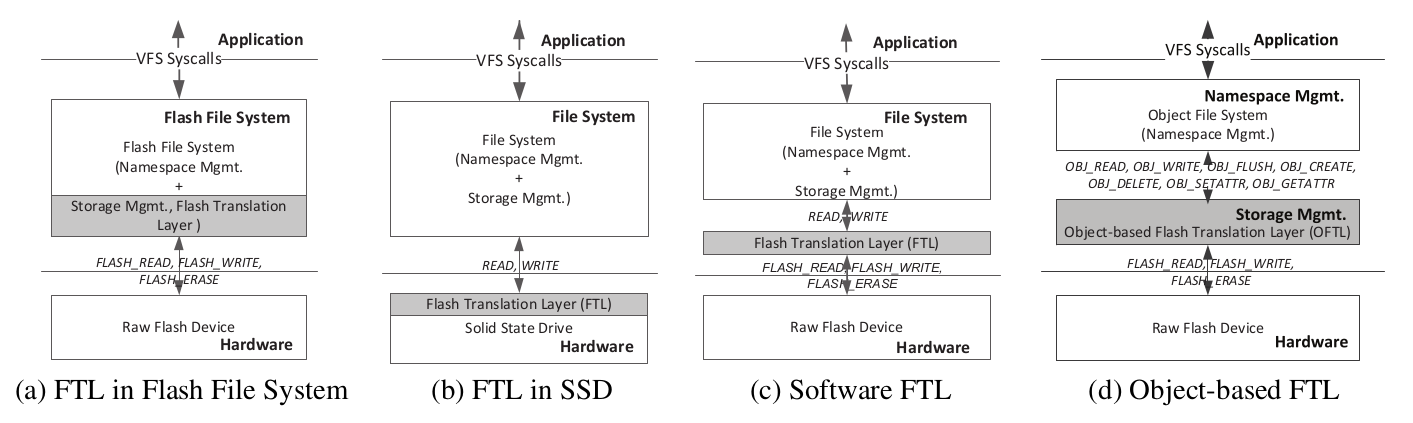
\includegraphics[width=0.8\textwidth]{translate_fig1.png}
  \caption*{图~1\hskip1em 基于闪存的文件系统结构}
\end{figure}

尽管基于软件的FTL比嵌入式FTL具有更好的性能,但文件系统和FTL之间的窄块接口阻止文件系统或FTL的优化。文件语义隐藏在狭窄的界面之后,阻碍了智能存储管理[35,26]。此外,闪存属性对文件系统不透明,导致文件系统优化失去了机会[20,29,28]。与基于对象的SCM [21]类似,我们提出了基于对象的FTL设计OFTL,以便与文件系统和闪存更好地配合,如图1(d)所示。在基于OFTL的体系结构中,存储管理从文件系统移动到OFTL以直接管理闪存,因此可以调查闪存属性以优化文件系统机制设计,如元数据同步的日志删除和频率降低。 OFTL通过读/写/擦除操作管理闪存,并直接访问每个闪存页面的页面元数据。另外,OFTL将字节单位访问接口导出到文件系统,这是一个基于对象的文件系统,不受存储管理的限制,只能管理名称空间。

\section{基于对象的闪存转换层}
基于OFTL的体系结构将存储空间管理从文件系统卸载到OFTL,以更好地协同设计文件系统和FTL。 OFTL访问页面单元接口中的原始闪存设备,同时将字节单元访问接口导出到文件系统。因此,OFTL将从每个对象的逻辑偏移量映射到Flash页面地址。在本节中,我们将描述OFTL接口和数据组织。

\begin{table}[htb]
    \centering
    \begin{minipage}[t]{0.8\linewidth}
    \caption*{表~1\hskip1em 对象接口}
      \begin{tabularx}{\linewidth}{lX}
        \toprule[1.5pt]
        {\heiti 操作} & {\heiti 描述} \\\midrule[1pt]
        \textbf{oread}(devid, oid, offset, len, buf) & 从编号为oid的对象的offset位置读取数据到buf\\
        \textbf{owrite}(devid, oid, offset, len, buf) & 向编号为oid的对象的offset位置写入buf中的数据\\
        \textbf{oflush}(devid, oid) & 将编号为oid的对象的数据和元数据持久化\\
        \textbf{ocreate}(devid, oid) & 创建编号为oid的对象\\
        \textbf{odelete}(devid, oid) & 删除编号为oid的对象\\
        \textbf{ogetattr}(devid, oid, buf) & 获取编号为oid的对象的标签\\
        \textbf{osetattr}(devid, oid, buf) & 设置编号为oid的对象的标签\\
        \bottomrule[1.5pt]
    \end{tabularx}
\end{minipage}
\end{table}

{\heiti OFTL接口。} OFTL将字节单位读/写接口导出到文件系统,以直接将访问大小以字节为单位传递给OFTL。表1显示了对象接口。 oread和owrite接口都将字节单位的偏移和len传递给OFTL,而不是扇区单元。因此,OFTL从应用程序中获得准确的访问大小,从而可以将小更新压缩成更少的页面,这在4.3节中讨论。另外,使用对象接口中提供的oid对每个对象进行操作,这使得OFTL知道所访问页面的数据类型。 OFTL利用对象语义对更新关联数据进行聚类。此外,OFTL使用类型语义区分数据页面的索引页面,以便在页面元数据中保留辅助元数据以实现懒惰索引,这在4.1节中讨论。
OFTL以页面单元读取/写入操作和块单位擦除操作访问闪存。页面元数据读/写可以在NVMe规范[6]之后直接从OFTL访问,该规范定义了用于访问PCI Express总线上的非易失性存储器的主机控制器接口。

\begin{figure}[h]
    \centering
    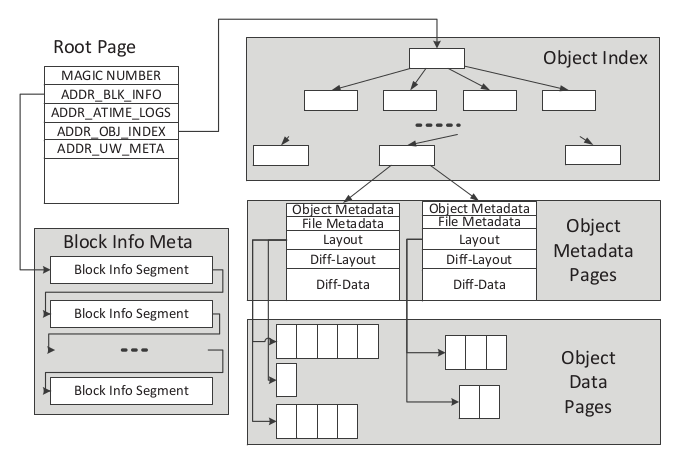
\includegraphics[width=0.8\textwidth]{translate_fig2.png}
    \caption*{图~2\hskip1em OFTL结构}
  \end{figure}

{\heiti 数据组织。 } OFTL由两个主要部分组成,对象存储和块信息元数据。单个根页面标识每个对象存储和块信息元数据的位置,如图2所示。对象存储分为三个级别:对象索引,对象元数据页面和对象数据页面。对象索引使用B +树将对象ID映射到其对象元数据。对象元数据包含传统上存储在文件系统索引节点中的信息,包括引用对象数据页面中的地址的分配信息。
块信息元数据保持每个闪存块的元数据信息,包括闪存块状态,无效页数(其数据过时但未被擦除)以及每个闪存块的擦除次数。每个闪存块有三种状态:FREE,UPDATING和USED,每个页面有三种状态:FREE,VALID和INVALID,这些在第4.2节中有解释。块信息元数据是以日志结构化的方式编写的。每个块信息条目有32位,其中20位用于擦除计数,10位用于无效页数,2位用于闪存块状态。块信息不是与每个闪存块一起存储,而是存储在闪存中的一个单独的空间中,这会在垃圾收集期间导致更少的页面更新。

\section{系统与闪存的协同设计}
OTFL使用三种技术来利用底层闪存设备的特性。在4.1节中,我们介绍了Backpointer-Assisted Lazy Indexing,这是一种有效维护数据和元数据之间一致性的机制。在4.2节中,我们介绍了我们的粗粒度块状态管理方法,它可以降低状态写入的频率。在第4.3节中,我们介绍了我们的压缩更新技术,该技术摊分了跨多个未对齐页面写入的页面写入成本。

\begin{figure}[h]
    \centering
    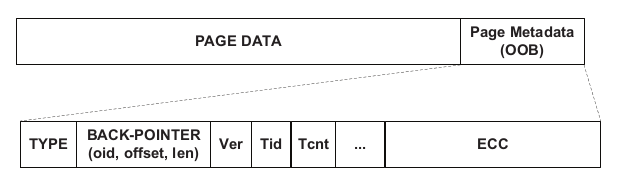
\includegraphics[width=0.8\textwidth]{translate_fig3.png}
    \caption*{图~3\hskip1em 页元数据}
  \end{figure}

\subsection{反向指针辅助的惰性索引}
索引元数据(对象元数据页面中用于指向数据页面的数据布局的指针或者指向对象索引以指向对象元数据页面的指针)应该同步写入以防存储设备损失或不一致。索引元数据的同步也称为索引持久性。虽然典型指针的大小为8个字节,但索引持久性会更新整个页面,即4KB或更大。因此,频繁的索引持久性导致严重的写入放大。

在索引元数据的惰性持久性中,在每个索引页面的页面元数据中采用了类型特定的反向指针技术,以减少索引持久化的频率,同时保持一致性。如图2所示,对象索引,对象元数据页面和对象数据页面在树结构中进行索引并形成三级分层结构。图3说明了页面元数据组织。在OFTL中,我们有两种类型的后向指示器(oid,offset,len)。一个用于数据页面来对对象元数据进行逆向索引,oid和offset,len分别表示对象id,对象中的逻辑页面偏移量和页面的有效数据长度。另一个用于对象元数据页面来反向索引对象索引,并且只有oid被设置为表示对象ID。在写入反指针时,首先设置类型以指示反指数的类型,以便可以针对不同类型正确理解反指针。我们也保留版本以确定最新的恢复页面版本。因此,类型特定的反向指针用作反向索引,并且索引持久化与页面更新解耦。

为了减少反向索引的扫描时间以在系统故障后重建索引元数据,我们使用更新窗口来跟踪最近分配的未完成索引元数据持久化的闪存块。更新窗口由检查点进程维护,检查点进程在更新窗口中的空闲页数低于阈值并且需要扩展窗口时触发。更新窗口描述了在发生故障后需要检查其反向索引的块集,因为索引可能不会引用它们。

更新窗口还提供多个页面的更新原子性。页面元数据保存事务信息(tid,tcnt),其中tid是每个写入操作的更新窗口中的唯一ID,tcnt是更新中页面的数量。对于写操作的所有页面,只有一个页面具有tcnt设置,其他页面的tcnt值为零。 tcnt用于在系统故障后检查操作的完整性。垃圾收集不允许在更新窗口中的闪存块上执行,以便完成原子性检查的事务信息。因此,使用闪存提供的写入原子可以消除日志。

在系统故障后重新启动时,扫描更新窗口中的对象数据页面。首先检查交易信息以确定涉及该页面的写入操作的完整性。如果写入不完整,则写入的所有页面都将被丢弃。这样就保证了原子性。在检查之后,如果在系统失败之前对象布局未被写入稳定,则读出后向指针以更新对象布局。由于所有更新都位于自上次检查点以来的更新窗口中,因此可以通过从当前更新窗口重新构建扫描页面中的后向指示器,将对象布局更新为最新版本。文件大小元数据也会随着所有有效数据大小的重新计算而更新。虽然其他描述性元数据(如修改时间和访问控制列表)在意外崩溃后可能会丢失,但系统一致性不会受到影响。类似地,可以用对象元数据页面的当前更新窗口的扫描来更新对象索引。通过页面元数据和更新窗口中的辅助信息,可以减少索引持久化频率,并提供写入原子性来消除日志。

\begin{figure}[h]
    \centering
    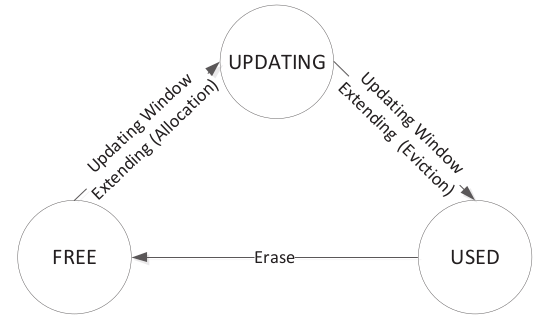
\includegraphics[width=0.8\textwidth]{translate_fig4.png}
    \caption*{图~4\hskip1em 闪存块的状态转换}
  \end{figure}

{\heiti 一致性和耐久性讨论。} 在懒惰索引技术中,系统崩溃后,除索引指针和大小之外的元数据可能会丢失。 这导致元数据的过时版本,这伤害元数据更新的持久性。 与耐久性相比,我们将一致性视为更重要的事情,因为索引的腐败会导致文件系统的不一致甚至失败。 我们使用懒惰索引技术来保证索引和大小可以在恢复期间重建。 但是对于持久性问题,我们选择让文件系统或应用程序确定让其他元数据持久化的时间,并显式同步。

\subsection{粗粒度块状态维护}
在闪存中,每个页面都有三种状态:FREE,VALID和INVALID。空闲页面是尚未写入的页面。有效页面是已写入的页面,其数据是有效数据。无效页面是已写入但其数据已过时的页面。有效和无效页面也称为INUSE页面。每个闪存块也有三种状态:FREE,UPDATING和USED。空闲块中的页面全部为空闲页面,已使用块中的页面全部处于使用页面中,而只有更新块同时具有空闲页面或未使用页面。由于页面是按顺序写入闪存块中的,因此最新分配的页码用于将空闲页面与更新块的使用中分开。因此,OFTL通过跟踪闪存块状态来区分空闲页面和使用中页面。对于inuse页面,索引元数据用于进一步区分有效页面和无效页面。有效页面在索引元数据中编入索引,而无效则不在索引中。因此,可以通过跟踪闪存块的状态来识别空闲,有效的无效页面,并且通过闪存块单元中的状态维护而不是页面单元来减少空闲空间管理成本。

OFTL通过降低元数据持久性的频率来进一步降低成本。闪存块状态的持久性仅在闪存块被分配给或从更新窗口驱逐出时执行,如图4的顶部所示。状态持久性被放宽,但是满足以下两个条件:(1)持久性空闲块是实际空闲块集的子集; (2)持续无效页面的数量不超过无效页面的实际数量。

第一个条件意味着一个空闲块可以被认为是非空闲的,这可能导致分配丢失。但是一个非空闲块不能被视为空闲,否则写入失败。它要求从FREE到UPDATING的状态转换立即刷新,但将状态持久性从USED释放到FREE。第二个条件放松了无效页面的数量持久性。无效页面的数量用于选择驱逐的闪存块并检查垃圾回收期间移动的有效页面的数量。通过检查索引元数据来区分有效页面和无效页面。在达到有效页面的数量之前,剩余的所有页面都是无效的,并且不再需要无效的页面检查,从而使被驱逐块的页面移动停止。在最坏的情况下,如果无效页面的持续数量少于实际数量,则必须检查所有页面。由于系统崩溃很少出现,所以对垃圾收集效率的影响是有限的。类似于无效页面的持续数量,记录的擦除次数可能会保持不变,这也可以接受,因为擦除次数不敏感。

总之,空闲空间管理从粗粒度块状态维护中受益,因为闪存块粒度状态跟踪和状态持久性的降低都减少了元数据成本。

\subsection{压缩更新}
通过字节单元访问接口,OFTL能够识别部分页面更新,这些页面更新只更新一页的一部分,既适用于小于一页的小型更新,也适用于大型更新的正面/反面。压缩更新技术压缩同一对象的部分页面更新,并将它们与其对象元数据页面共同定位以减少更新页面。

\begin{figure}[h]
    \centering
    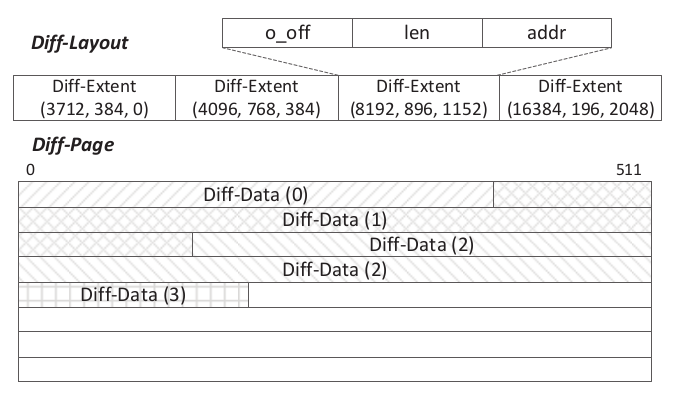
\includegraphics[width=0.8\textwidth]{translate_fig5.png}
    \caption*{图~5\hskip1em Differential Layout(Diff-Layout)数据结构}
  \end{figure}

{\heiti 部分页面更新。} OFTL中的部分页面更新被压缩并插入差异页面,又名差异页面。存储在diff-page中的每个数据段都称为diff-data。 Diff-data使用三元组<ooff,len,addr>进行diff-extent索引,其中ooff和len分别表示对象偏移量和diffdata的长度,addr是diff-数据在diff-页。 Diff-extents在diff-layout中按照对象偏移量的升序保持不变。每个对象都有一个diff-layout,它是一个对象的所有diff-extents的集合。图5显示了数据结构。

尽管部分页面更新被吸收到差异页面中,而差异页面在差异布局中编入索引,但整个页面更新会直接写入对象页面。对象页面在布局中进行索引,这是一个对象的所有范围的集合,用于保存完整页面的起始地址和长度对。与差异布局一样,布局也记录在对象元数据页面中,如图2所示。在压缩更新技术中,读取,写入和合并操作如下所述:

\begin{itemize}
    \item 写入:写入数据分为多页。不开始或结束页面对齐的部分被标识为部分页面更新,而其他部分则被认定为整页更新。然后部分页面更新在diff-pages中更新。因为部分更新总是取代整个页面,所以整个页面更新必须使相应的差异数据无效并删除其差异范围,然后更新布局以引用整个页面。
    \item 合并:当差异页面已满时需要合并操作。合并时,会扫描diff-extents以选择在diff-pages中消耗最多空间的驱逐的逻辑页面。然后读取驱逐的逻辑页面的对象页面并与diff-data合并。之后,合并的页面被写入新的对象页面,并且相应的diff-data和diff-extents被删除。
    \item 读取:首先以不同的格式检查读取操作。如果它在diff-data中被满足,则读缓冲区被diff-data填充。否则,读取对象页面并与任何现有的对应diff-data合并。
\end{itemize}

{\heiti 更新协同定位。} 在大多数情况下,每个对象的元数据大小远小于页面大小。 OFTL不是压缩多个对象的元数据,而是与对象元数据页面不同的页面。 由于每个数据更新之后都有元数据更新,例如文件大小或修改时间,因此diff-data和元数据页面的共同位置通常会节省一页写入。 在协同定位中,diff-page的大小小于一个页面大小,并且取决于对象元数据的大小更改。 diff-page的大小是通过从flash页面大小中减去元数据大小来计算的,flash页面大小用于检查diff-page是否已满。 一旦完成,触发合并操作以选择一些diffdata并将它们合并到对象数据页面。 通过这种方式,部分页面更新的成本通过压缩和协同定位来分摊。

\section{实现}
我们在Linux内核3.2.9中实现OFTL作为内核模块。该模块由三层组成:转换层,缓存层和存储层。

转换层遵循图2所示的设计。使用Log-Structured Merge Tree(LSM-Tree)[27]实现闪存对象索引,该索引具有用于快速查找的内存B +树并添加记录每个对象索引更新的<operation,object ID,phy addr>。每个对象都有一个内存中对象的元数据数据结构,它记录访问统计信息和两个基于范围的布局,以及图2所示的闪存对象元数据页面。diff-layout和layout都链接它们的范围在内存中的列表结构中。在写入请求上,写入数据首先分页对齐。整页更新被写入数据页面,然后进行布局更新,而部分页面更新被插入diff-data,然后是diff-layout更新。对象操作转换为元数据或数据页面上的读/写操作并转发到缓存层。

元数据和数据页面缓存在缓存层中。 OFTL缓存遵循linux内核中页面缓冲区的设计,不同之处在于替换是用整个对象完成的。在写操作时,如果设置了SYNC标志,则高速缓存检查SYNC标志并从存储层调用闪存写入接口。否则,更新缓存层中的对象缓存。页面分配被延迟直到页面需要刷新。然后,缓存层从更新窗口分配空闲页面并调用闪存写入接口以通过存储层写入页面。

存储层从缓存层接收闪存读/写/擦除操作,构建bio请求,并将它们发送到通用块层。我们使用系统中的TRIM / DISCARD命令和SATA协议来执行擦除操作。 OOB的DMA传输遵循NVMe标准中的设计[6]。由于硬件限制,目前在存储器中模拟OOB操作。

\begin{figure}[h]
    \centering
    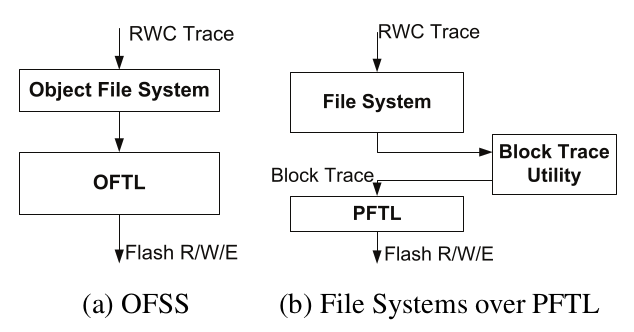
\includegraphics[width=0.8\textwidth]{translate_fig6.png}
    \caption*{图~6\hskip1em Trace驱动的模拟框架}
  \end{figure}

在OFTL中,我们使用简单的垃圾收集和磨损平衡策略。当空闲块的百分比下降到15%以下时开始垃圾收集,并一直持续到百分比超过该值。在耗损均衡中,擦除次数的上限用于防止闪存块擦除次数过多。在平均擦除次数增加后,这一上限会周期性地上升。我们将在未来纳入更好的战略。

为了评估其他文件系统解决方案,我们还实现了一个简单的目标文件系统来解析命名空间,如图1(d)所示。目标文件系统使用内存中的哈希表来保持从路径到对象ID的映射,并通过将对象ID替换为路径将IO请求传递给OFTL。我们在评估部分调用基于OFTL的系统对象闪存存储系统(OFSS)。

\section{评估}
我们测量写入放大率,写入闪存的总大小/计数,除以应用程序发出的写入总大小/计数,以评估OFSS的写入效率以及ext3,ext2和btrfs最新的页面级FTL。

在本节中,我们首先评估这四个系统的总体性能,然后分析元数据放大。我们还测量闪存页面大小的影响以及扩展OFTL设计带来的更新窗口的开销。

\begin{table}[htb]
    \centering
    \begin{minipage}[t]{0.8\linewidth}
    \caption*{表~2\hskip1em 工作负载特性}
      \begin{tabularx}{\linewidth}{lXXXX}
        \toprule[1.5pt]
        {\heiti 负载名称} & {\heiti 写次数} & {\heiti 写大小(KB)} & {\heiti 刷新次数} & {\heiti 不对齐写的百分比} \\\midrule[1pt]
        iPhoto & 496542 & 6651962 & 37054 & 51.2\%\\
        iPages & 75661 & 183728 & 565 & 99.6\%\\
        LASR-1 & 32249 & 42600 & 1714 & 93.3\%\\
        LASR-2 & 111531 & 216114 & 14998 & 99.0\%\\
        LASR-3 & 21956 & 24426 & 3056 & 96.1\%\\
        TPC-C & 26144 & 219689 & 489 & 7.1\%\\
        \bottomrule[1.5pt]
    \end{tabularx}
\end{minipage}
\end{table}

\subsection{实验设置}
我们从系统级IO跟踪中提取读取,写入和关闭操作(RWC跟踪)并在文件系统和OFSS上重放它们。图6显示了tracedriven仿真框架。在重放程序中,关闭操作会在文件系统中执行fsync操作或在OFSS中执行对象刷新操作。在OFSS中,我们将I / O的数量和大小收集到OFTL存储层的闪存中。在文件系统评估中,我们使用blktrace实用程序[1]在文件系统评估中捕获存储设备上的I / O,然后在PFTL上重播块跟踪,PFTL是在Linux kernel-3.2中作为内核模块实现的模拟页级FTL。 9。我们收集PFTL中闪存的I / O数量和大小。在仿真中,PFTL使用类似于主存储器管理的两级页表将逻辑页号转换为物理页号。 LazyFLT [23]功能集成到PFTL中以减少映射开销。

我们评估桌面环境中iBench [19]的两个工作负载,服务器环境中LASR [5]的三个一个月跟踪以及数据库管理系统中的一个TPCC跟踪。 TPC-C跟踪是使用strace实用程序[8]从运行在PostgreSQL上的DBT2工作负载[3]收集的。表2列出了六项工作量的特点。

实验在SUSE Linux 11.1上进行,Linux内核3.2.9在4核Intel Xeon X5472 3GHz处理器和8GB内存的计算机上运行。除用于操作系统的磁盘驱动器外,还使用Seagate 7200rpm ST31000524AS磁盘驱动器进行跟踪收集。在实验中,ext3和ext2使用noatime,nodiratime选项进行挂载,而btrfs使用ssd,discard和lzo选项进行挂载。在OFSS设置中,默认页面大小为4KB,闪存块大小为256KB。对象数据和元数据的更新窗口都设置为64个闪存块的大小。默认的OFTL缓存大小为32MB。

\subsection{总体比较}

\begin{figure}[h]
    \centering
    \caption*{表~3\hskip1em 写放大的整体评估}
    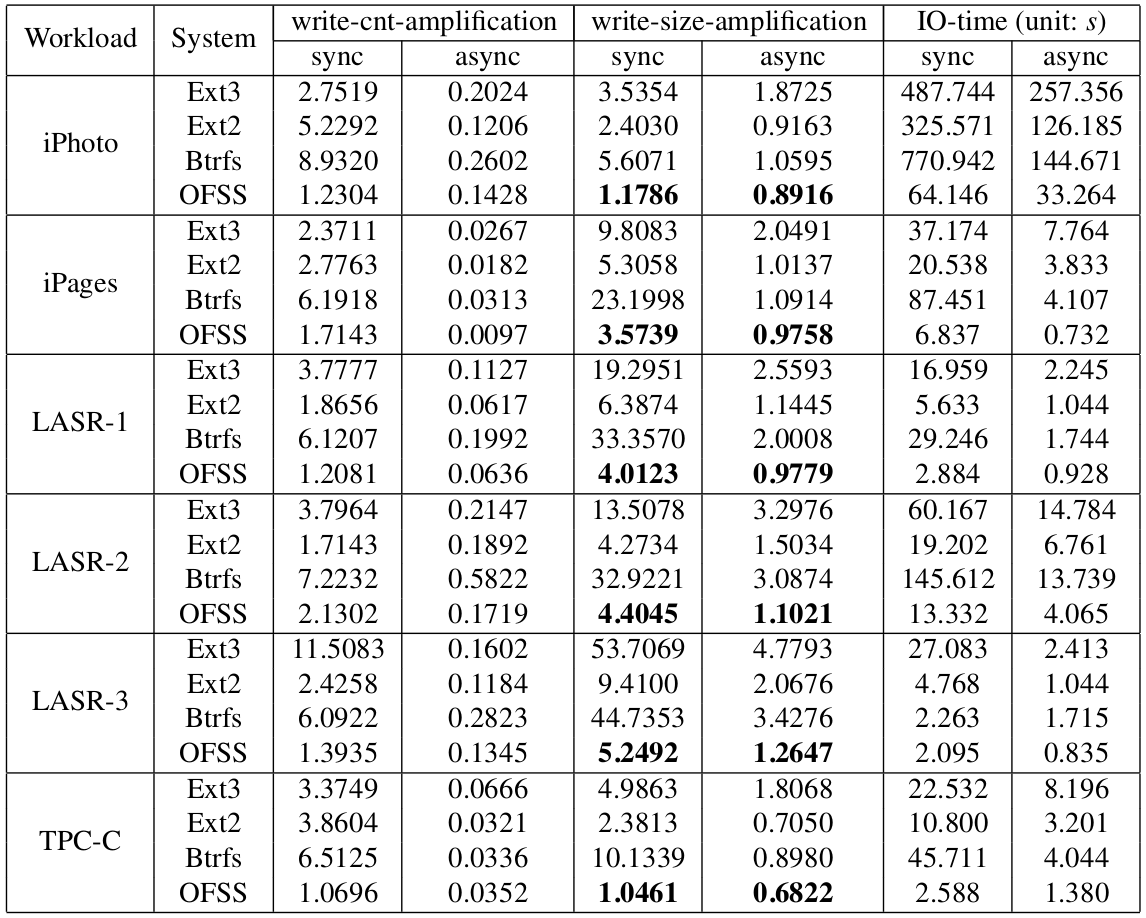
\includegraphics[width=0.8\textwidth]{translate_tab3.png}
  \end{figure}

在本节中,针对建立在PFTL上的ext2,ext3和btrfs,针对OFSS评估写入效率和IO时间。为了提供数据一致性,ext3使用数据日志选项装载,而btrfs使用写入时复制来更新数据,而ext2则不提供一致性。 OFSS通过利用闪存的不覆盖属性并将事务信息保存在页面元数据中来提供数据一致性。这四个系统以SYNC和ASYNC模式进行评估。在SYNC模式下,数据和元数据在请求返回之前需要刷新稳定。 Ext2和ext3使用同步选项安装以支持SYNC模式。 Btrfs在文件打开操作中使用O SY NC标志,因为btrfs中不支持sync安装选项。在ASYNC模式下,数据和元数据被缓存在内存中,直到显式同步,时间到期或缓存逐出。三个文件系统的默认挂载选项支持ASYNC模式。

表3显示了在SYNC模式下每个系统的总写入次数和写入大小所测得的写入放大倍数。写入计数在ext3,ext2,btrfs和OFSS中的平均写入放大倍数分别为4.60,2.98,6.85和1.11。写入大小的写入放大显示类似的结果,并且ext3,ext2,btrfs和OFSS中的平均值分别为17.47,5.03,24.99和2.64。差异主要来自与写入操作相关的元数据成本。在ext2中,写操作具有数据更新,inode更新的子操作,并且如果需要空间分配,则有时会更新位图。在使用数据日志的ext3中,数据和元数据复制到日志日志中,然后进行提交/异常同步写入,稍后通过日志守护进程对实际位置进行检查点设置。即使写入计数在ext3和ext2中由于合并写入而在检查点中接近,由于在日志日志中添加了重复的数据和元数据,ext3中的写入大小仍然远远大于ext2中的写入大小。在SYNC模式下,btrfs将更新记录到特殊的日志树中以消除整个系统更新[30],从而导致写入放大率高。 Btrfs针对性能进行了优化,它使用“ssd”分配方案进行免寻找分配,并且尚未针对闪存耐久性进行优化[2]。随着杂志的淘汰,元数据同步频率的降低和压缩更新,OFSS相对于其他三种传统文件系统的写入放大率降低了47.4%〜89.4%。

如表3所示,ASYNC模式下的写入放大率分别为0.13,0.09,0.23和0.09,写入次数分别为2.73,1.23,1.93和0.98,写入大小分别为ext3,ext2,btrfs和OFSS。在ASYNC模式下,写入放大并不像SYNC模式那样糟糕。原因是元数据同步不频繁,元数据更新在缓冲区以及数据中合并。但是,由于日志记录,ext3中的写入强度加倍。 Btrfs必须更新用于写入时复制更新机制的索引元数据,消耗更多页面。此外,当页面未对齐时,页面对齐的更新机制会浪费空间,这会对所有三个传统文件系统产生写入放大效果。相比之下,与三个传统文件系统相比,OFSS性能更好,写入放大率降低了19.8%〜64.0%。

总体IO时间也显示在表3中以进行性能比较。由于硬件限制,我们通过向SSD发出请求而不是原始闪存来评估性能。由于我们设计的重点是写入放大减少而非映射策略的性能导向设计,垃圾收集或耗损均衡,因此SSD内部的FTL对性能评估影响不大。我们收集和累积每次操作的设备I / O时间,这是从操作到SSD的问题到SSD的确认的度量。如图所示,两种模式下的OFSS性能都明显优于其他模式。写入大小的减少不仅延长了闪存存储的使用寿命,而且还提高了性能。此外,性能改进部分来自基于对象的FTL设计,该设计使用OFTL缓存中的延迟空间分配来实现更好的I / O调度。

{\heiti 工作量讨论。} 一般而言,OFSS为拥有大量页面未对齐更新或频繁数据同步的工作负载带来更大的好处。当同步写入操作时,传统文件系统需要多个页面,包括数据,inode和位图文件系统块的页面才能更新。元数据开销对小更新很重要,其中只更新了几个字节。平均更新大小小于1KB的LASR-1和LASR3工作负载在SYNC模式下暴露了无法接受的写入放大,而OFSS极大地减少了元数据开销,并且使得放大率更低。由于压缩更新技术,未对齐的页面更新也可以从OFSS中受益。一个反例是TPC-C工作负载,它在用户空间中拥有自己的缓冲区,并以页为单位写入数据。 OFSS对TPC-C工作负载的改进不如其他工作负载那么重要。

\subsection{元数据的写放大}

\begin{figure}[h]
    \centering
    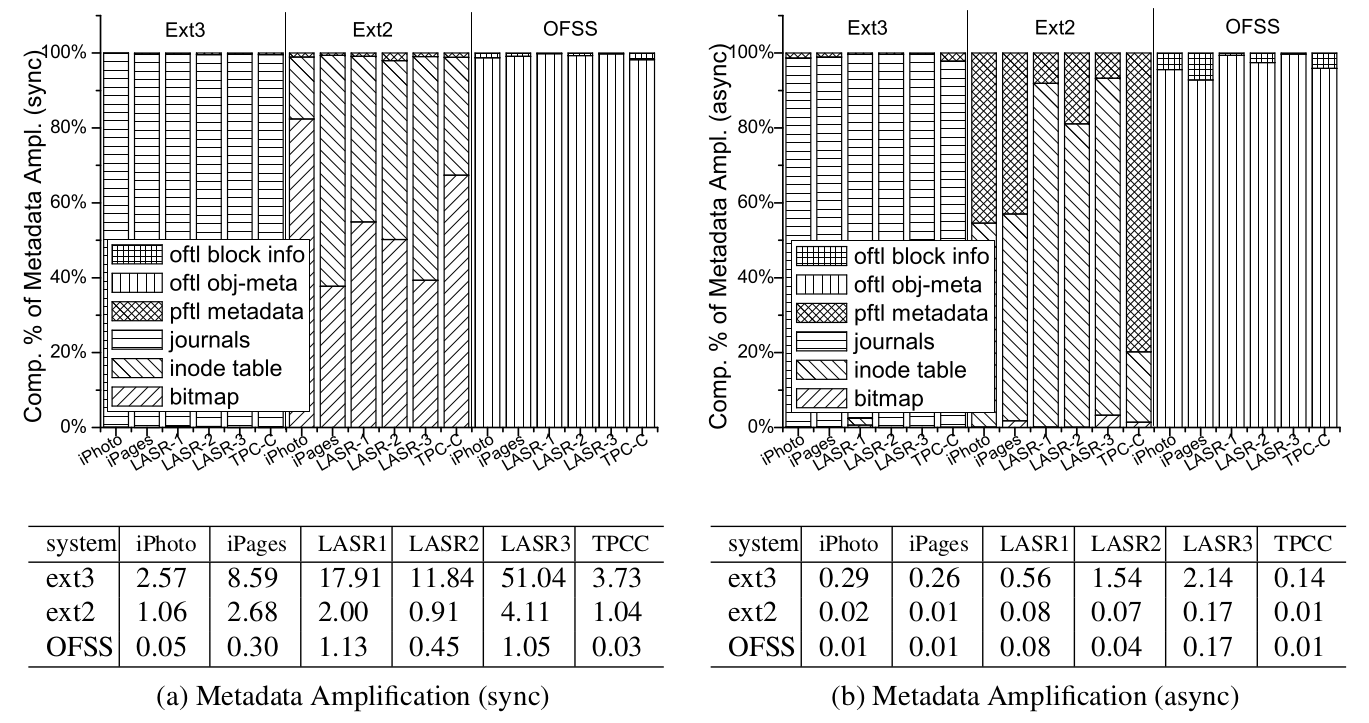
\includegraphics[width=0.8\textwidth]{translate_fig7.png}
    \caption*{图~7\hskip1em 元数据的写放大}
  \end{figure}

为了进一步了解OFSS的改进以及期刊移除和元数据同步缩减的效果,我们仔细研究元数据放大。在评估中,我们通过使用dump2 f s命令的转储信息检查ext2和ext3的物理布局来识别每个访问的文件系统块类型。日志类型由块跟踪中的“k日志”标识。我们从此分析中忽略了btrfs,因为我们无法区分块跟踪中写入地址的元数据和数据更新。图7显示了表格中的总元数据放大率以及SYNC和ASYNC模式中表格上方的各种元数据的百分比。

从图7中,ext3的元数据放大有两个观察。一个是与文件系统元数据的写入放大相比,PFTL的写入放大可以忽略不计。另一个原因是日志显着地放大了写入并且控制了成本。 ext2和ext3之间的区别验证了日志删除的好处。在下文中,我们将通过将OFSS与ext2进行比较来进一步了解减少元数据同步的好处。

在元数据同步减少评估中,我们在计算OFTL的元数据放大时,从OFSS中的元数据页面中去除差异数据。如图7(a)所示,inode和bitmap更新消耗了SYNC模式中大部分的放大。 inode更新的写入放大率从平均值ext2中的0.99降至OFTL元数据更新所测量的OFSS中的0.50。好处不仅来自懒惰索引,而且来自使用压缩更新的已摊销元数据页更新成本。文件系统块位图更新的写入放大率从平均ext2中的0.93降低到用OFTL闪存块信息更新测量的OFSS中的0.0019,其显示了粗粒度块状态维护的益处。由于空闲空间是以闪存块单位进行管理的,实验中为64页(256KB),比ext2中的4KB块大得多,因此粗粒度块状态维护极大地有利于自由空间管理。

在如图7(b)所示的ASYNC模式下,inode和元数据更新成本分别是ext2和OFSS的主要成本。他们两人的写入放大成本平均在0.05左右。传统文件系统将多个inode压缩到一个inode表文件系统块中,与OFSS中的压缩更新技术相比,这是一种减少元数据放大的不同方法。这两种方法在ASYNC模式下都有类似的效果。 ext2中的文件系统块位图在ASYNC模式下进行缓存和合并,使成本接近OFSS中的闪存块状态维护成本。

\subsection{闪存页面大小的影响}

\begin{figure}[h]
    \centering
    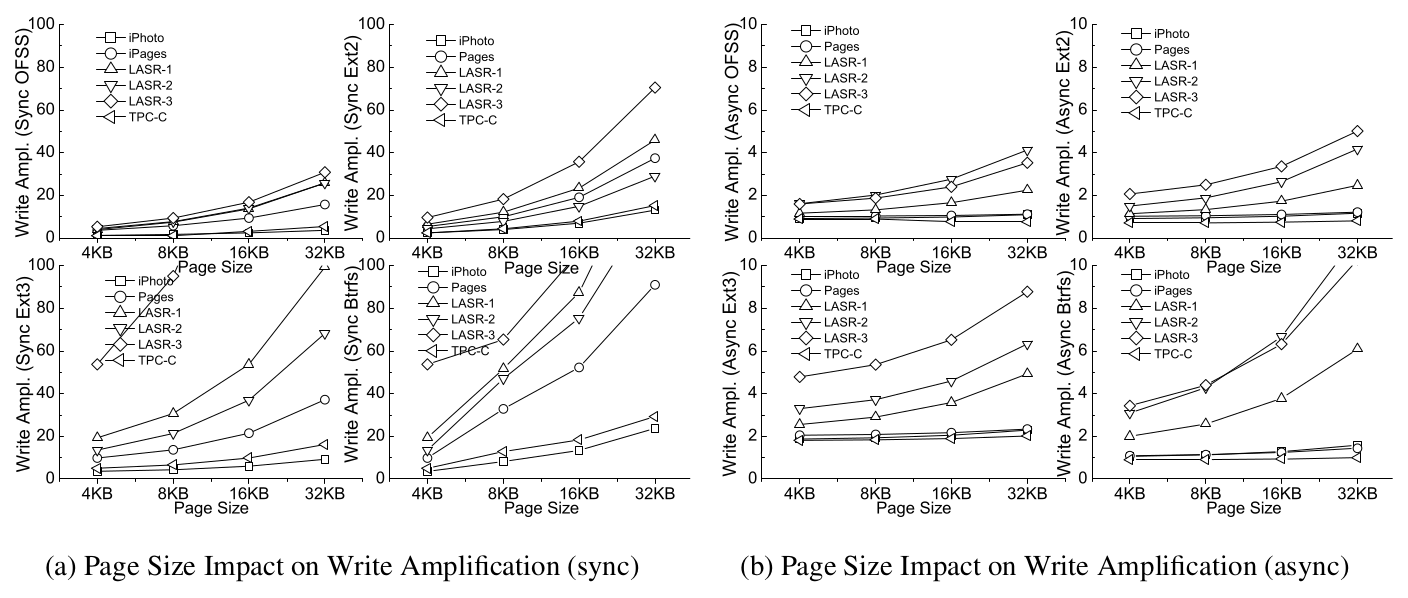
\includegraphics[width=0.8\textwidth]{translate_fig8.png}
    \caption*{图~8\hskip1em 闪存页大小对写放大的影响}
  \end{figure}

闪存页面的大小已经暴露出闪存制造的增长趋势[17]。我们用4KB,8KB,16KB和32KB不同页面大小评估ext2,ext3,btrfs和OFSS的写入效率。由于ext2和ext3支持4KB的最大文件系统块大小,并且当lead / node / sector大小设置为8KB或更高时,btrfs不稳定,所以我们将4KB块跟踪访问与PFTL中不同的Flash页面大小对齐以供评估。如图8所示,随着传统文件系统中页面大小的增加,写入放大率显着增加,而OFSS显示出显着的改进。 LASR-1和LASR-3等小访问大小的工作负载的恶化速度要快得多。另一个观察结果是,当Flash页面大小增加时,如图8(a)所示的SYNC模式下的写入放大比图8(b)所示的ASYNC差很多。这是因为在大多数情况下,SYNC模式下的访问大小远小于页面大小。相比之下,ASYNC模式下的访问被缓存并合并为更大的请求。 OFSS中的压缩更新技术进一步压缩了部分页面更新并将它们与元数据共同定位,以减少要更新的页面,从而提高页面利用率。因此,OFSS在SYNC模式下的写入放大效果更好,大约为30,在ext3中接近9%,ASYNC模式下的写入放大接近3,在btrfs中接近25%。

\subsection{扩展更新窗口的开销}

\begin{figure}[h]
    \centering
    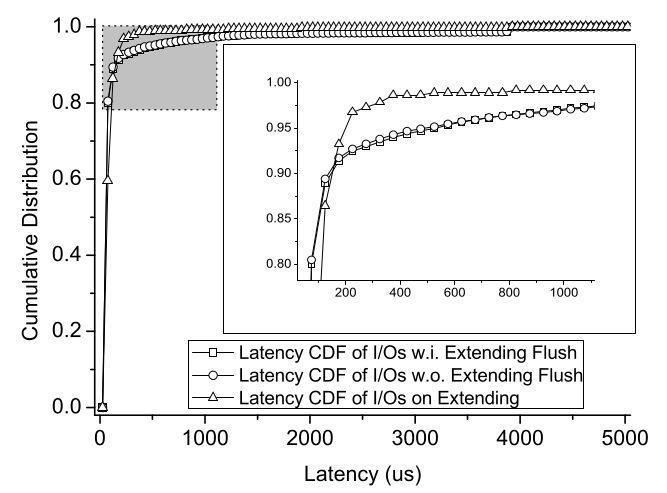
\includegraphics[width=0.8\textwidth]{translate_fig9.png}
    \caption*{图~9\hskip1em 扩展更新窗口的开销}
  \end{figure}

更新窗口用于减少系统崩溃后的扫描时间,但由于扩展更新窗口时存在索引持久性而导致额外写入。为了评估开销,我们收集了每个操作的I / O延迟的两个数据集,一个用于正常扩展,另一个用于没有索引持久性的扩展。两个数据集中潜伏期的累积分布用图9中几乎相同的线描绘,显示了接近的性能。我们还会在扩展期间识别I / O并收集每个I / O的延迟时间,以显示对外部I / O延迟的影响。扩展期间I / O的延迟与所有I / O的平均值相差不大。在该图的放大部分中,即使延迟I / O的累积分布在延迟小于200us时比平均增长慢,当延迟大约为200us时,其增长得更快。结果,扩展的I / O中有99.6%的延迟小于400us。此外,扩展操作很少出现,只有0.04%的I / O满足扩展。因此,我们得出结论:扩展更新窗口对性能的影响有限。

\section{相关工作}
Flash文件系统[32,10,9]利用闪存的nooverwrite属性进行日志结构更新,通过直接管理闪存来优化性能。但除了磨损平衡之外,他们对闪光耐力没有太大的贡献。无名写入[35]和直接文件系统[20]建议删除文件系统的映射,以允许FTL管理存储空间以提高性能。但是文件语义无法传递给FTL进行智能存储空间管理。 OFTL采用基于对象的存储的概念[25]将对象接口导出到文件系统,从而轻松地将文件语义传递到设备以进行智能数据布局。

最近的研究还提出消除闪存中日志造成的重复写入。 Write Atomic [28]通过利用FusionIO ioDrives中VSL [4]的基于日志的结构导出原子写入接口。 TxFlash [29]在页面元数据的帮助下使用循环提交协议来导出相同的接口。但是,循环属性维护起来很复杂,并且该协议在故障后需要进行全驱动扫描。相比之下,OFTL采用与日志结构文件系统[31]中的事务支持类似的简单协议,将事务信息保存在页面元数据中,并在更新窗口中跟踪最近更新的闪存块以便快速恢复。

在磁盘存储系统中使用反向指针来避免在Backlog中移动文件系统块时的文件系统元数据更新[24],或者通过将后向指针嵌入数据块,目录条目和Backpointerbased一致性中的inode来提供后续一致性检查[16] 。在基于闪存的存储中,LazyFTL [23]建议通过在页面元数据中保留逻辑页面编号(LPN)作为反向指针,并将页面记录在更新闪存块区域中,来懒惰地更新页面级FTL的映射条目,以块级FTL为代价提供页面级FTL的性能。但它不会触及文件系统中的元数据,这对写入放大作出了很大贡献。相反,OFTL利用页面元数据优化系统设计,并使用反向指针作为索引元数据惰性持久性的反向索引。

CAFTL [15]和DeltaFTL [33]合并冗余数据并压缩FTL中的相似页面,而LFS [13],JFFS2 [32],UBIFS [9]和btrfs [2]压缩文件中的数据页系统。他们都通过利用页面内容相似性来使用压缩,这与使用OFTL中访问大小信息的压缩更新技术正交。 IPL(页内记录)[22]采用类似于OFTL的方法,并在每个闪存块中保留一个日志区域以吸收小的更新。但是,如果数据和元数据页面分布在多个闪存块中,则会受到同步写入的影响。 reiserfs [7]中的尾部打包与OFTL中的压缩更新技术最相关。 Reiserfs将每个文件的尾部包装在其inode中。 OFTL与OFTL以不覆盖的方式更新不同,因此OFTL不仅压缩尾部,而且压缩每个写入操作的头部,包括追加和更新操作。

\section{结论}
传统文件系统专注于顺序存取优化,而不是写入放大缩小,这对闪存非常重要。系统机制(如日志记录,元数据同步和页面对齐更新)极大地放大了写入强度,而间接性带来的透明性阻止了系统利用闪存特性。在本文中,我们提出了一个基于对象的设计名称OFTL,其中存储管理从文件系统卸载到FTL以直接管理闪存。页面元数据用于保留延迟索引的反向索引和事务信息,以便为日志删除提供写入原子性,借助更新窗口跟踪尚未检查点的最新分配的闪存块。另外,空闲空间管理可以跟踪闪存块状态而不是页面状态,并降低状态持久化的频率以进一步降低元数据成本。使用字节单位访问接口,OFTL中标识的部分页面更新被压缩并与元数据共存以减少更新。在系统与闪存共同设计的情况下,文件系统的写入放大显著减少。

\section*{致谢}
我们要感谢我们的指导者Margo Seltzer和匿名审稿人提出的富有洞察力的意见和详细的建议,这大大改进了本文的内容和陈述。 我们也感谢Shuai Li在实验装置方面的帮助,Guangyu Sun在演讲中的帮助。 本研究由国家自然科学基金(批准号:60925006),国家自然科学基金重点项目(批准号:61232003),国家高技术研究发展计划(批准号: 2013AA013201),清华腾讯互联网创新技术联合实验室研究基金支持。

% \section*{参考文献}

% \begin{translationbib}
% \item blktrace(8) - linux man page. http://linux.die.net/man/8/blktrace.
% \item Btrfs. http://btrfs.wiki.kernel.org.
% \item Dbt2 test suite. http://sourceforge.net/apps/mediawiki/osdldbt.
% \item Fusionio virtual storage layer. http://www/fusionio.com/products/vsl.
% \item Lasr system call io trace. http://iotta.snia.org/tracetypes/1.
% \item The nvm express standard. http://www.nvmexpress.org.
% \item Reiserfs. http://reiser4.wiki.kernel.org.
% \item strace(1) - linux man page. http://linux.die.net/man/1/strace.
% \item Ubifs - ubi file-system. http://www.linux-mtd.infradead.org/doc/ubifs.html.
% \item Yaffs. http://www.yaffs.net.
% \item N. Agrawal, V. Prabhakaran, T. Wobber, J. D. Davis, M. Manasse, and R. Panigrahy. Design tradeoffs for ssd performance. In Proceedings of USENIX 2008 Annual Technical Conference, 2008.
% \item S. Boboila and P. Desnoyers. Write endurance in flash drives: measurements and analysis. In Proceedings of the 8th USENIX conference on File and storage technologies (FAST), 2010.
% \item Michael Burrows, Charles Jerian, Butler Lampson, and Timothy Mann. On-line data compression in a log-structured file system. In Proceedings of the fifth international conference on Architectural support for programming languages and operating systems (ASPLOS), 1992.
% \item L.P. Chang. On efficient wear leveling for large-scale flash-memory storage systems. In Proceedings of the 2007 ACM symposium on Applied computing, 2007.
% \item F. Chen, T. Luo, and X. Zhang. Caftl: A content-aware flash translation layer enhancing the lifespan of flash memory based solid state drives. In Proceedings of the 9th USENIX conference on File and Storage Technologies (FAST), 2011.
% \item V. Chidambaram, T. Sharma, A. C. Arpaci-Dusseau, and R. H. Arpaci-Dusseau. Consistency without ordering. In Proceedings of the 10th USENIX conference on File and Storage Technologies (FAST), 2012.
% \item L. M. Grupp, J. D. Davis, and S. Swanson. The bleak future of nand flash memory. In Proceedings of the 10th USENIX conference on File and Storage Technologies (FAST), 2012.
% \item L.M. Grupp, A.M. Caulfield, J. Coburn, S. Swanson, E. Yaakobi, P.H. Siegel, and J.K. Wolf. Characterizing flash memory: anomalies, observations, and applications. In Proceedings of the 42nd Annual IEEE/ACM International Symposium on Microarchitecture (MICRO-42), 2009.
% \item T. Harter, C. Dragga, M. Vaughn, A. C. Arpaci-Dusseau, and R. H. Arpaci-Dusseau. A file is not a file: understanding the i/o behavior of apple desktop applications. In Proceedings of the 23rd ACM Symposium on Operating Systems Principles (SOSP), 2011.
% \item W. K. Josephson, L. A. Bongo, D. Flynn, and K. Li. Dfs: a file system for virtualized flash storage. In Proceedings of the 8th USENIX conference on File and Storage Technologies (FAST), 2010.
% \item Y. Kang, J. Yang, and E. L. Miller. Object-based scm: An efficient interface for storage class memories. In Proceedings of IEEE 27th Symposium on Mass Storage Systems and Technologies (MSST), 2011.
% \item S. W. Lee and B. Moon. Design of flash-based dbms: an in-page logging approach. In Proceedings of the 2007 ACM SIGMOD International Conference on Management of Data (SIGMOD), 2007.
% \item D. Ma, J. Feng, and G. Li. Lazyftl: A page-level flash translation layer optimized for nand flash memory. In Proceedings of the 2011 International Conference on Management of Data (SIGMOD), 2011.
% \item P. Macko, M. Seltzer, and K.A. Smith. Tracking back references in a write-anywhere file system. In Proceedings of the 8th USENIX conference on File and storage technologies (FAST), 2010.
% \item M. Mesnier, G.R. Ganger, and E. Riedel. Object-based storage. IEEE Communications Magazine, 41(8):84–90, 2003.
% \item D. Nellans, M. Zappe, J. Axboe, and D. Flynn. ptrim ()+ exists (): Exposing new ftl primitives to applications. In 2nd Annual Non-Volatile Memory Workshop, 2011.
% \item P. O’Neil, E. Cheng, D. Gawlick, and E. O’Neil. The log-structured merge-tree (lsm-tree). Acta Informatica, 33(4):351–385, 1996.
% \item X. Ouyang, D. Nellans, R. Wipfel, D. Flynn, and D. K. Panda. Beyond block i/o: Rethinking traditional storage primitives. In Proceedings of the 17th IEEE International Symposium on High Performance Computer Architecture (HPCA), 2011.
% \item V. Prabhakaran, T. L. Rodeheffer, and L. Zhou. Transactional flash. In Proceedings of the 8th USENIX conference on Operating Systems Design and Implementation (OSDI), 2008.
% \item O. Rodeh, J. Bacik, and C. Mason. Btrfs: The linux b-tree filesystem. Technical report, IBM Almaden Reserach Center, 2012.
% \item M. Seltzer. Transaction support in a log-structured file system. In Proceedings of the Ninth International Conference on Data Engineering, 1993.
% \item David Woodhouse. Jffs2: The journalling flash file system, version 2. http://sourceware.org/jffs2.
% \item G. Wu and X. He. Delta-ftl: improving ssd lifetime via exploiting content locality. In Proceedings of the 7th ACM European Conference on Computer Systems (EuroSys), 2012.
% \item Q. Yang and J. Ren. I-cash: Intelligently coupled array of ssd and hdd. In Proceedings of the 17th IEEE International Symposium on High Performance Computer Architecture (HPCA), 2011.
% \item Y. Zhang, L. P. Arulraj, A. C. Arpaci-Dusseau, and R. H. Arpaci-Dusseau. De-indirection for flash-based ssds with nameless writes. In Proceedings of the 10th USENIX conference on File and Storage Technologies (FAST), 2012.
% \end{translationbib}

\title{书面翻译对应的原文索引}
\begin{translationbib}
\item Lu Y, Shu J, Zheng W, et al. Extending the lifetime of flash-based storage through reducing write amplification from file systems.[C]//FAST: volume 13. 2013.
\end{translationbib}

\end{appendix}

%% 个人简历
% \begin{resume}

  \resumeitem{个人简历}

  xxxx 年 xx 月 xx 日出生于 xx 省 xx 县。

  xxxx 年 9 月考入 xx 大学 xx 系 xx 专业,xxxx 年 7 月本科毕业并获得 xx 学士学位。

  xxxx 年 9 月免试进入 xx 大学 xx 系攻读 xx 学位至今。

  \researchitem{发表的学术论文} % 发表的和录用的合在一起

  % 1. 已经刊载的学术论文(本人是第一作者,或者导师为第一作者本人是第二作者)
  \begin{publications}
    \item Yang Y, Ren T L, Zhang L T, et al. Miniature microphone with silicon-
      based ferroelectric thin films. Integrated Ferroelectrics, 2003,
      52:229-235. (SCI 收录, 检索号:758FZ.)
    \item 杨轶, 张宁欣, 任天令, 等. 硅基铁电微声学器件中薄膜残余应力的研究. 中国机
      械工程, 2005, 16(14):1289-1291. (EI 收录, 检索号:0534931 2907.)
    \item 杨轶, 张宁欣, 任天令, 等. 集成铁电器件中的关键工艺研究. 仪器仪表学报,
      2003, 24(S4):192-193. (EI 源刊.)
  \end{publications}

  % 2. 尚未刊载,但已经接到正式录用函的学术论文(本人为第一作者,或者
  %    导师为第一作者本人是第二作者)。
  \begin{publications}[before=\publicationskip,after=\publicationskip]
    \item Yang Y, Ren T L, Zhu Y P, et al. PMUTs for handwriting recognition. In
      press. (已被 Integrated Ferroelectrics 录用. SCI 源刊.)
  \end{publications}

  % 3. 其他学术论文。可列出除上述两种情况以外的其他学术论文,但必须是
  %    已经刊载或者收到正式录用函的论文。
  \begin{publications}
    \item Wu X M, Yang Y, Cai J, et al. Measurements of ferroelectric MEMS
      microphones. Integrated Ferroelectrics, 2005, 69:417-429. (SCI 收录, 检索号
      :896KM)
    \item 贾泽, 杨轶, 陈兢, 等. 用于压电和电容微麦克风的体硅腐蚀相关研究. 压电与声
      光, 2006, 28(1):117-119. (EI 收录, 检索号:06129773469)
    \item 伍晓明, 杨轶, 张宁欣, 等. 基于MEMS技术的集成铁电硅微麦克风. 中国集成电路,
      2003, 53:59-61.
  \end{publications}

  \researchitem{研究成果} % 有就写,没有就删除
  \begin{achievements}
    \item 任天令, 杨轶, 朱一平, 等. 硅基铁电微声学传感器畴极化区域控制和电极连接的
      方法: 中国, CN1602118A. (中国专利公开号)
    \item Ren T L, Yang Y, Zhu Y P, et al. Piezoelectric micro acoustic sensor
      based on ferroelectric materials: USA, No.11/215, 102. (美国发明专利申请号)
  \end{achievements}

\end{resume}


%% 本科生进行格式审查是需要下面这个表格,答辩可能不需要。选择性留下。
% 综合论文训练记录表
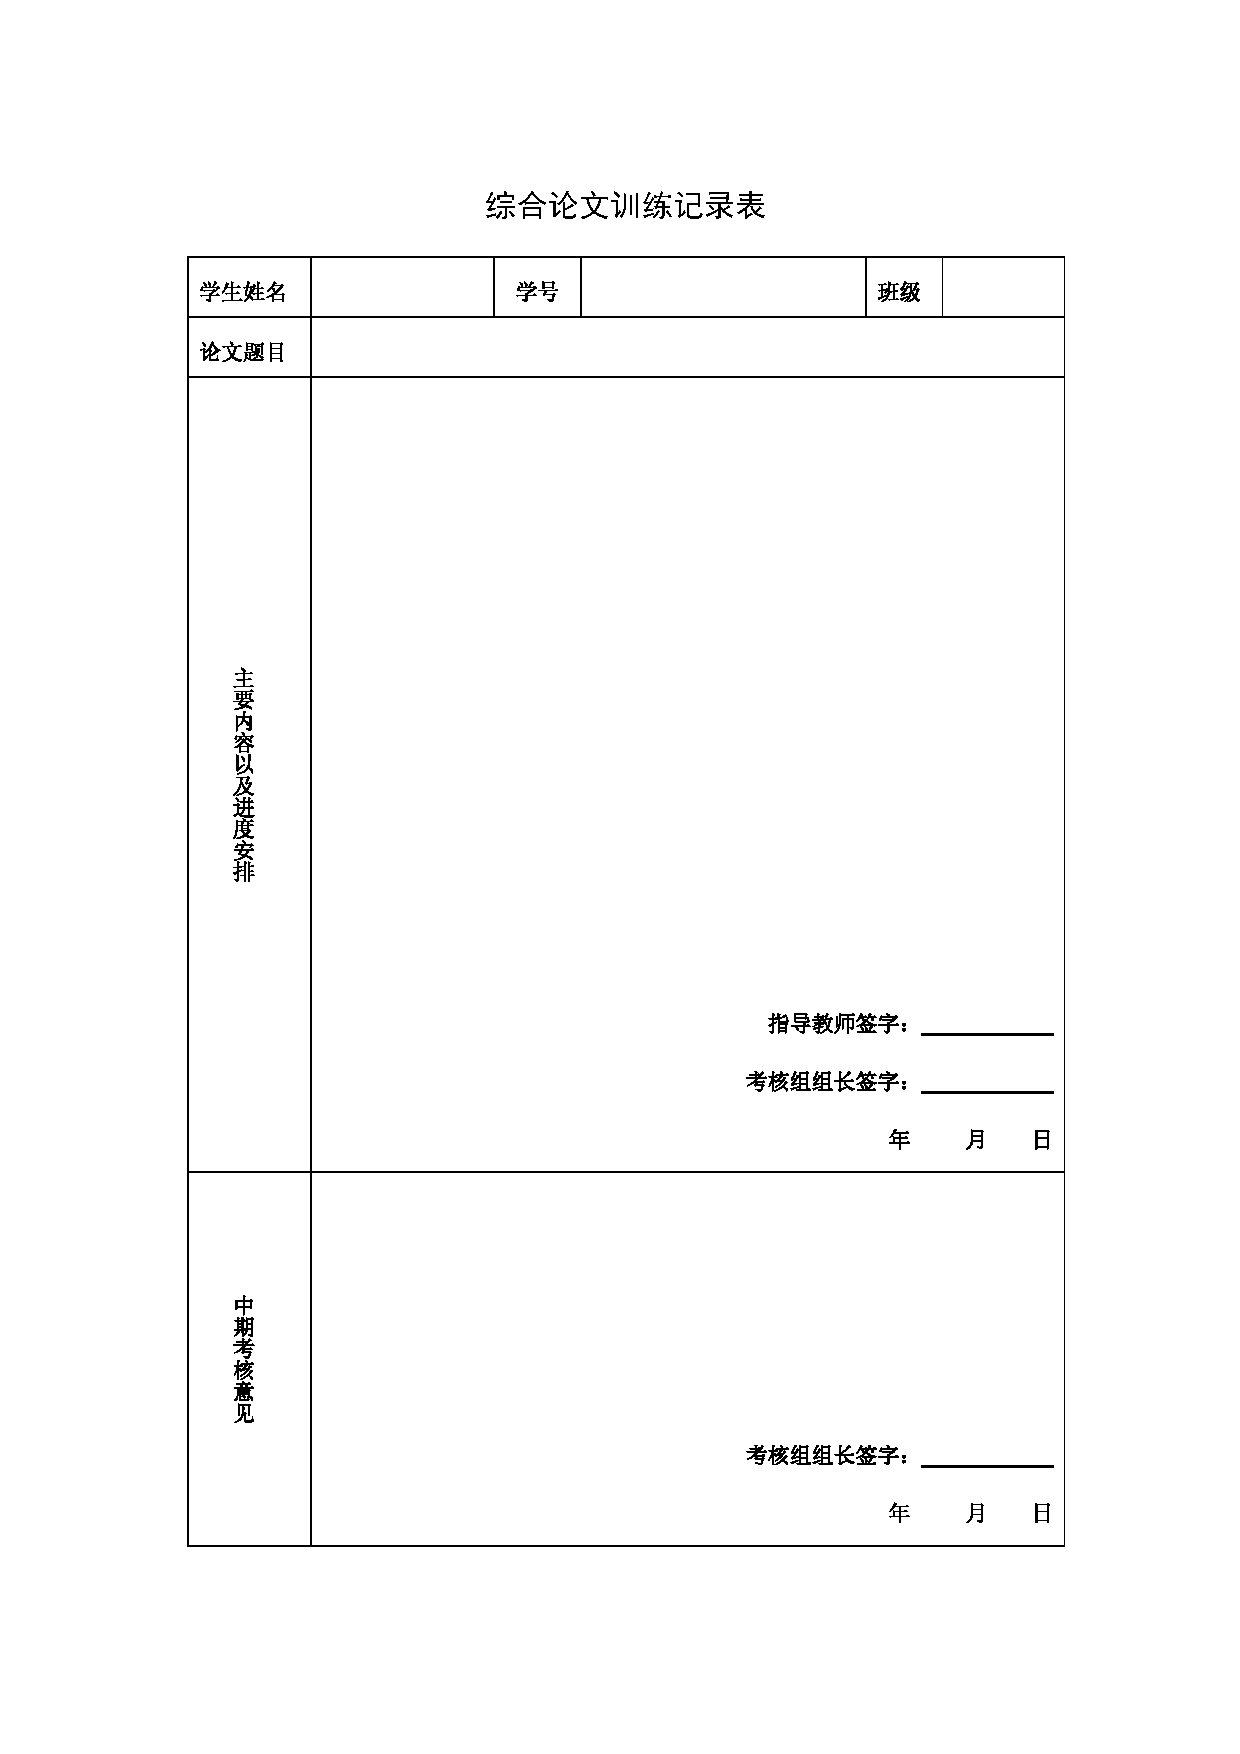
\includepdf[pages=-]{scan-record.pdf}
\end{document}
